% ECPM paper, single-file version generated from the Overleaf project.
% Needs acl.sty, acl_natbib.bst and references.bib beside it.
% Tables and number macros are generated; edit the project sources and regenerate rather than editing here.
\documentclass[11pt]{article}

% "review" for submission (anonymous, line numbers); "final" for camera-ready.
\usepackage[review]{acl}

\usepackage{times}
\usepackage{latexsym}
\usepackage[T1]{fontenc}
\usepackage[utf8]{inputenc}
\usepackage{microtype}
\IfFileExists{inconsolata.sty}{\usepackage{inconsolata}}{}
\usepackage{graphicx}
\usepackage{amsmath,amssymb}
\usepackage{booktabs}
\usepackage{tabularx}
\usepackage{multirow}
\usepackage{array}
\usepackage[table]{xcolor}
\usepackage{tikz}
\usetikzlibrary{arrows.meta,positioning,calc,fit,backgrounds}
\usepackage{pgfplots}
\pgfplotsset{compat=1.17}
\usepackage{subcaption}
\usepackage{adjustbox}
\usepackage{placeins}
\usepackage[capitalise,noabbrev]{cleveref}
% Indicator symbol used in the formal definition (from Paper.tex).
\IfFileExists{bbm.sty}{\usepackage{bbm}}{}
\providecommand{\mathbbm}{\mathbf}
% Cross-references to appendix sections print "Appendix A", not "Section A".
\makeatletter
\g@addto@macro\appendix{\crefalias{section}{appendix}\crefalias{subsection}{appendix}}
\makeatother

% ===== begin macros.tex =====
% Palette. Orange marks the intervention target, blue the off-route control.
\definecolor{ecTarget}{HTML}{C8502A}
\definecolor{ecControl}{HTML}{1F5FA0}
\definecolor{ecRoute}{HTML}{3D3D3A}
\definecolor{ecMuted}{HTML}{8C8A82}
\definecolor{ecLine}{HTML}{B4B2A9}
\definecolor{ecFill}{HTML}{F4F3EF}
\definecolor{ecShade}{HTML}{FAECE7}
\definecolor{ecTrans}{HTML}{0F6E56}
% Evidence families in fig:refs. Hue is what a reference reads (success rates, outcome
% distributions, generator knowledge), lightness within a family is complexity. Validated with
% the dataviz palette checker (light, all pairs): CVD dE >= 13.0, normal-vision dE >= 16.3.
\definecolor{ecRefRate}{HTML}{2A78D6}
\definecolor{ecRefTrans}{HTML}{1BAF7A}
\definecolor{ecRefBayes}{HTML}{00785A}
\definecolor{ecRefGen}{HTML}{4A3AA7}

% Notation. Symbols from the draft are kept, symbols from Vafa et al. are added.
\newcommand{\Tstar}{T^{*}}
\newcommand{\Ustar}{U^{*}}
\newcommand{\act}[1]{a_{#1}}
\newcommand{\pa}[2]{\mbox{$(\mathrm{#1},\,a_{#2})$}}
\newcommand{\nd}[1]{\mathrm{#1}}
\newcommand{\goesto}{\,{\to}\,}

% Drafting markers. Values that depend on runs not yet made, and facts the
% team still has to supply, are shown in grey so they stay visible without
% reading as errors. Set \drafttrue to \draftfalse before submission: any
% marker left in the text then stops the build.
\newif\ifdraft \drafttrue
\definecolor{ecPending}{HTML}{8C8A82}
% \RES is a model-result slot, filled from run artifacts by the results step.
% It prints a grey small-caps "run": the value is computed by the repo pipeline from the run artifacts.
% PH and pending mark anything else and stop every non-draft build.
% \resallowedtrue (set by check_build.sh nores) builds with result slots open.
\newif\ifresallowed \resallowedfalse
\ifdraft
  \newcommand{\PH}{{\color{ecPending}\textsc{tbd}}}
  \newcommand{\RES}{{\color{ecPending}\textsc{run}}}
  \newcommand{\pending}[1]{{\color{ecPending}\textit{[pending: #1]}}}
\else
  \newcommand{\PH}{\errmessage{Unfilled placeholder}}
  \ifresallowed
    \newcommand{\RES}{{\color{ecPending}\textsc{run}}}
  \else
    \newcommand{\RES}{\errmessage{Unfilled result slot}}
  \fi
  \newcommand{\pending}[1]{\errmessage{Pending item: #1}}
\fi
\newcommand{\TODO}[1]{\pending{#1}}
\newcommand{\PENDING}[1]{\pending{#1}}
% ===== end macros.tex =====

% ===== begin figures/numbers.tex =====
% Generated by scripts/make_numbers.py. Do not edit by hand.
\newcommand{\nSeedsEight}{84}
\newcommand{\nSeedsSixteen}{80}
\newcommand{\nDegMove}{60}
\newcommand{\nDegRestraint}{24}
\newcommand{\nDetTies}{72}
\newcommand{\nHeldEight}{80}
\newcommand{\nHeldSixteen}{72}
\newcommand{\nInstSto}{504}
\newcommand{\nInstDet}{420}
\newcommand{\pctOverTau}{39}
\newcommand{\pctOverBand}{3}
\newcommand{\pctBayesDetSB}{90.0}
\newcommand{\pctRateDetSB}{90.0}
\newcommand{\locRateSBFive}{0.76}
\newcommand{\locGenSBFive}{0.99}
\newcommand{\locRateDegFive}{0.20}
\newcommand{\locGenDegFive}{0.40}
\newcommand{\locRateRedFive}{0.08}
\newcommand{\locGenRedFive}{0.99}
\newcommand{\locRateSBTen}{0.93}
\newcommand{\locGenSBTen}{1.00}
\newcommand{\locRateDegTen}{0.51}
\newcommand{\locGenDegTen}{0.65}
\newcommand{\locRateRedTen}{0.08}
\newcommand{\locGenRedTen}{1.00}
\newcommand{\locRateSBTwenty}{1.00}
\newcommand{\locGenSBTwenty}{1.00}
\newcommand{\locRateDegTwenty}{0.75}
\newcommand{\locGenDegTwenty}{0.88}
\newcommand{\locRateRedTwenty}{0.07}
\newcommand{\locGenRedTwenty}{1.00}
\newcommand{\pctGenRedMin}{99}
\newcommand{\routeRefSB}{0.86}
\newcommand{\routeRefDeg}{0.58}
\newcommand{\postFailFour}{0.78}
\newcommand{\postFailFive}{0.92}
\newcommand{\postFailSix}{0.97}
\newcommand{\mdePaired}{0.16}
\newcommand{\nAgentic}{51}
\newcommand{\linksMin}{14}
\newcommand{\linksMax}{18}
\newcommand{\postSixLo}{0.966}
\newcommand{\postSixHi}{0.973}
\newcommand{\postFiveLo}{0.906}
\newcommand{\postFiveHi}{0.926}
% ===== end figures/numbers.tex =====

% ===== begin figures/derived_numbers.tex =====
% Generated by figscripts/gen_numbers.py. Do not edit by hand.
\newcommand{\bcRateStoSilentbreakCI}{(5,0.76) += (0,0.079) -= (0,0.101) (10,0.93) += (0,0.038) -= (0,0.075) (20,1.00) += (0,-0.000) -= (0,0.044)}
\newcommand{\bcGenStoSilentbreakCI}{(5,0.99) += (0,0.008) -= (0,0.051) (10,1.00) += (0,-0.000) -= (0,0.044) (20,1.00) += (0,-0.000) -= (0,0.044)}
\newcommand{\bcRateStoDegradationCI}{(5,0.20) += (0,0.098) -= (0,0.072) (10,0.51) += (0,0.104) -= (0,0.105) (20,0.75) += (0,0.080) -= (0,0.102)}
\newcommand{\bcGenStoDegradationCI}{(5,0.40) += (0,0.107) -= (0,0.098) (10,0.65) += (0,0.093) -= (0,0.107) (20,0.88) += (0,0.053) -= (0,0.087)}
\newcommand{\bcRateStoRedirectCI}{(5,0.08) += (0,0.078) -= (0,0.041) (10,0.08) += (0,0.078) -= (0,0.041) (20,0.07) += (0,0.075) -= (0,0.038)}
\newcommand{\bcGenStoRedirectCI}{(5,0.99) += (0,0.008) -= (0,0.051) (10,1.00) += (0,-0.000) -= (0,0.044) (20,1.00) += (0,-0.000) -= (0,0.044)}
\newcommand{\exN}{23}
\newcommand{\exSBDet}{11}
\newcommand{\exSBLoc}{6}
\newcommand{\exNCFalse}{5}
\newcommand{\exNCRouteOpt}{5}
\newcommand{\exCellLocOpt}{3}
\newcommand{\exCellLocOnly}{3}
\newcommand{\exCellOptOnly}{6}
\newcommand{\exCellNeither}{11}
\newcommand{\exOR}{1.77}
\newcommand{\exORlo}{0.30}
\newcommand{\exORhi}{10.35}
\newcommand{\exFisherP}{0.64}
\newcommand{\redirNbNoChangeRate}{33}
\newcommand{\redirNbBreakRate}{8}
\newcommand{\redirNbNoChangeTrans}{1}
\newcommand{\redirNbBreakTrans}{63}
% ===== end figures/derived_numbers.tex =====
% ===== begin figures/ref_k10.tex =====
% Generated by paper/make_fig_refs.py from runs/references/part_sto_10.json. Do not edit by hand.
% Rows (y): 6 irrelevant, 5 silent break, 4 hard removal, 3 redirect, 2 degradation (route moves), 1 degradation (restraint).
\newcommand{\figRefRate}{(0.988,5.76) += (0.010,0) -= (0.052,0) (0.929,4.76) += (0.038,0) -= (0.076,0) (1.000,3.76) += (0.000,0) -= (0.044,0) (0.083,2.76) += (0.079,0) -= (0.042,0) (0.500,1.76) += (0.123,0) -= (0.123,0) (0.542,0.76) += (0.179,0) -= (0.191,0)}
\newcommand{\figRefTrans}{(0.988,5.92) += (0.010,0) -= (0.052,0) (0.929,4.92) += (0.038,0) -= (0.076,0) (1.000,3.92) += (0.000,0) -= (0.044,0) (0.976,2.92) += (0.017,0) -= (0.059,0) (0.500,1.92) += (0.123,0) -= (0.123,0) (0.542,0.92) += (0.179,0) -= (0.191,0)}
\newcommand{\figRefBayes}{(0.988,6.08) += (0.010,0) -= (0.052,0) (0.952,5.08) += (0.029,0) -= (0.069,0) (1.000,4.08) += (0.000,0) -= (0.044,0) (1.000,3.08) += (0.000,0) -= (0.044,0) (0.450,2.08) += (0.125,0) -= (0.119,0) (0.542,1.08) += (0.179,0) -= (0.191,0)}
\newcommand{\figRefGen}{(1.000,6.24) += (0.000,0) -= (0.044,0) (1.000,5.24) += (0.000,0) -= (0.044,0) (1.000,4.24) += (0.000,0) -= (0.044,0) (1.000,3.24) += (0.000,0) -= (0.044,0) (0.667,2.24) += (0.106,0) -= (0.126,0) (0.625,1.24) += (0.163,0) -= (0.198,0)}
% ===== end figures/ref_k10.tex =====
% ===== begin figures/queried_restricted.tex =====
% Generated by paper/fill_offline.py from runs/references/queried_restricted.json. Do not edit by hand.
\newcommand{\nQueriedTarget}{41}
\newcommand{\nQueriedSeeds}{84}
\newcommand{\qrRate}{0.95}
\newcommand{\qrBayes}{0.98}
\newcommand{\qrGen}{1.00}
% ===== end figures/queried_restricted.tex =====
% ===== begin figures/reference_agent.tex =====
% Generated by paper/fill_offline.py from runs/references/offline_numbers.json. Do not edit by hand.
\newcommand{\lagRefAgent}{2.5}
\newcommand{\nLagRefAgent}{44}
\newcommand{\nLagRefSeeds}{51}
% ===== end figures/reference_agent.tex =====
% ===== begin tables/model_settings.tex =====
% Generated by paper/gen_model_settings.py RUNS_DIR from run artifacts. Open slots are \RES until the runs exist.
\newcommand{\mGemmaQuant}{\RES{}}
\newcommand{\mGemmaRuntime}{\RES{}}
\newcommand{\mAccessGemma}{\RES{}}
\newcommand{\mGPTfourSnapshot}{\RES{}}
\newcommand{\mAccessGPTfour}{\RES{}}
\newcommand{\mAccessSol}{\RES{}}
\newcommand{\mDeepSeekThinking}{\RES{}}
\newcommand{\mDeepSeekProvider}{\RES{}}
\newcommand{\mAccessDeepSeek}{\RES{}}
\newcommand{\mAccessKimi}{\RES{}}
% ===== end tables/model_settings.tex =====

% ===== begin figures/transcribed_numbers.tex =====
% pctOldFalseAlarm is regenerated by paper/fill_offline.py (runs/baseline_k_sweep_seeds1-30.json).
% verified by paper/fill_offline.py; no run artifact found in the repository.
% Replace with generated values before camera-ready (see CHANGELOG, unverified list).
\newcommand{\pctOldFalseAlarm}{17}
% ===== end figures/transcribed_numbers.tex =====

% ===== begin figures/baseline_curves_data.tex =====
% Generated by scripts/reference_sweep.py. Do not edit by hand.
\newcommand{\bcRateStoSilentbreak}{(5,0.76) (10,0.93) (20,1.00)}
\newcommand{\bcTransStoSilentbreak}{(5,0.76) (10,0.93) (20,1.00)}
\newcommand{\bcBayesStoSilentbreak}{(5,0.79) (10,0.95) (20,1.00)}
\newcommand{\bcRateStoHardremoval}{(5,1.00) (10,1.00) (20,1.00)}
\newcommand{\bcTransStoHardremoval}{(5,1.00) (10,1.00) (20,1.00)}
\newcommand{\bcBayesStoHardremoval}{(5,1.00) (10,1.00) (20,1.00)}
\newcommand{\bcRateStoRedirect}{(5,0.08) (10,0.08) (20,0.07)}
\newcommand{\bcTransStoRedirect}{(5,0.85) (10,0.98) (20,1.00)}
\newcommand{\bcBayesStoRedirect}{(5,0.88) (10,1.00) (20,1.00)}
\newcommand{\bcRateStoDegradation}{(5,0.20) (10,0.51) (20,0.75)}
\newcommand{\bcTransStoDegradation}{(5,0.21) (10,0.51) (20,0.75)}
\newcommand{\bcBayesStoDegradation}{(5,0.21) (10,0.48) (20,0.71)}
\newcommand{\bcRateStoIrrelevant}{(5,0.79) (10,0.99) (20,1.00)}
\newcommand{\bcTransStoIrrelevant}{(5,0.79) (10,0.99) (20,1.00)}
\newcommand{\bcBayesStoIrrelevant}{(5,0.80) (10,0.99) (20,1.00)}
\newcommand{\bcRateDetSilentbreak}{(5,1.00) (10,1.00) (20,1.00)}
\newcommand{\bcTransDetSilentbreak}{(5,1.00) (10,1.00) (20,1.00)}
\newcommand{\bcBayesDetSilentbreak}{(5,1.00) (10,1.00) (20,1.00)}
\newcommand{\bcRateDetHardremoval}{(5,1.00) (10,1.00) (20,1.00)}
\newcommand{\bcTransDetHardremoval}{(5,1.00) (10,1.00) (20,1.00)}
\newcommand{\bcBayesDetHardremoval}{(5,1.00) (10,1.00) (20,1.00)}
\newcommand{\bcRateDetRedirect}{(5,0.10) (10,0.10) (20,0.10)}
\newcommand{\bcTransDetRedirect}{(5,1.00) (10,1.00) (20,1.00)}
\newcommand{\bcBayesDetRedirect}{(5,1.00) (10,1.00) (20,1.00)}
\newcommand{\bcRateDetIrrelevant}{(5,1.00) (10,1.00) (20,1.00)}
\newcommand{\bcTransDetIrrelevant}{(5,1.00) (10,1.00) (20,1.00)}
\newcommand{\bcBayesDetIrrelevant}{(5,1.00) (10,1.00) (20,1.00)}
% ===== end figures/baseline_curves_data.tex =====

% ===== begin figures/baseline_curves_data_n16.tex =====
% Generated by scripts/reference_sweep.py. Do not edit by hand.
\newcommand{\bcSixteenRateStoSilentbreak}{(5,0.84) (10,0.95) (20,1.00)}
\newcommand{\bcSixteenTransStoSilentbreak}{(5,0.84) (10,0.95) (20,1.00)}
\newcommand{\bcSixteenBayesStoSilentbreak}{(5,0.85) (10,0.96) (20,1.00)}
\newcommand{\bcSixteenRateStoHardremoval}{(5,1.00) (10,1.00) (20,1.00)}
\newcommand{\bcSixteenTransStoHardremoval}{(5,1.00) (10,1.00) (20,1.00)}
\newcommand{\bcSixteenBayesStoHardremoval}{(5,1.00) (10,1.00) (20,1.00)}
\newcommand{\bcSixteenRateStoRedirect}{(5,0.00) (10,0.03) (20,0.01)}
\newcommand{\bcSixteenTransStoRedirect}{(5,0.88) (10,0.97) (20,1.00)}
\newcommand{\bcSixteenBayesStoRedirect}{(5,0.90) (10,1.00) (20,1.00)}
\newcommand{\bcSixteenRateStoDegradation}{(5,0.30) (10,0.36) (20,0.72)}
\newcommand{\bcSixteenTransStoDegradation}{(5,0.30) (10,0.36) (20,0.71)}
\newcommand{\bcSixteenBayesStoDegradation}{(5,0.28) (10,0.38) (20,0.69)}
\newcommand{\bcSixteenRateStoIrrelevant}{(5,0.78) (10,0.95) (20,0.99)}
\newcommand{\bcSixteenTransStoIrrelevant}{(5,0.78) (10,0.95) (20,0.99)}
\newcommand{\bcSixteenBayesStoIrrelevant}{(5,0.80) (10,0.99) (20,1.00)}
\newcommand{\bcSixteenRateDetSilentbreak}{(5,1.00) (10,1.00) (20,1.00)}
\newcommand{\bcSixteenTransDetSilentbreak}{(5,1.00) (10,1.00) (20,1.00)}
\newcommand{\bcSixteenBayesDetSilentbreak}{(5,1.00) (10,1.00) (20,1.00)}
\newcommand{\bcSixteenRateDetHardremoval}{(5,1.00) (10,1.00) (20,1.00)}
\newcommand{\bcSixteenTransDetHardremoval}{(5,1.00) (10,1.00) (20,1.00)}
\newcommand{\bcSixteenBayesDetHardremoval}{(5,1.00) (10,1.00) (20,1.00)}
\newcommand{\bcSixteenRateDetRedirect}{(5,0.05) (10,0.05) (20,0.05)}
\newcommand{\bcSixteenTransDetRedirect}{(5,1.00) (10,1.00) (20,1.00)}
\newcommand{\bcSixteenBayesDetRedirect}{(5,1.00) (10,1.00) (20,1.00)}
\newcommand{\bcSixteenRateDetIrrelevant}{(5,1.00) (10,1.00) (20,1.00)}
\newcommand{\bcSixteenTransDetIrrelevant}{(5,1.00) (10,1.00) (20,1.00)}
\newcommand{\bcSixteenBayesDetIrrelevant}{(5,1.00) (10,1.00) (20,1.00)}
% ===== end figures/baseline_curves_data_n16.tex =====

% ===== begin figures/generator_curves_data.tex =====
% Generated from figures/generator_sweep.json (scripts/generator_sweep.py). Do not edit by hand.
\newcommand{\bcGenStoSilentbreak}{(5,0.99) (10,1.00) (20,1.00)}
\newcommand{\bcGenStoDegradation}{(5,0.40) (10,0.65) (20,0.88)}
\newcommand{\bcGenStoRedirect}{(5,0.99) (10,1.00) (20,1.00)}
% ===== end figures/generator_curves_data.tex =====

% ===== begin figures/knowing_doing_data.tex =====
% Generated by scripts/make_tables.py. Do not edit by hand.
% superseded by tables/belief_use.tex
% ===== end figures/knowing_doing_data.tex =====


\title{Reporting a Change and Acting on It:\\
Language Models against Evidence-Only Observers}

\author{Anonymous ACL submission}

\begin{document}
\maketitle

% ####################################################################
% #                           MAIN PAPER                             #
% #  ARR: at most 8 pages of content (long paper). Limitations and   #
% #  the ethics statement follow the content and do not count.       #
% ####################################################################

% ===== begin sections/00_abstract.tex =====
\begin{abstract}
A language model that routes well after its environment changes may not have noticed the change, and a model that reports a change may not act on it. We separate these in a controlled routing world. Each instance pairs two worlds that differ in at most one link. The model reads observation logs from before the change and commits to a route and to beliefs. It then reads logs from after the change and reports whether anything changed, where, what it now believes about each link, and how it would route. In an agentic arm the model acts step by step instead. We read every answer against evidence-only observers that see exactly what the model sees, so that a failure can be attributed to the model rather than to the logs. Across five models and two graph families, \RES. When the counts are tabulated for them, \RES. Models that state that a link no longer works still route through it in \RES\ of cases, and in the agentic arm they choose a link after six observed failures of it in \RES\ of such choices.
\end{abstract}
% ===== end sections/00_abstract.tex =====

% ===== begin sections/01_introduction.tex =====
\section{Introduction}\label{sec:intro}
Language models are increasingly asked to act in environments that change while they work: a tool stops responding, a link in a network fails, an action now leads somewhere else. Acting well afterwards requires noticing the change, locating it, and acting on what one now believes. Task success is weak evidence that any of this happened~\cite{vafa2024}, and a model's stated reasoning need not match what drives its output~\cite{turpin2023}. A model that routes around a failure may have located it, or may have planned on the latest evidence alone. A model that reports a failure may still route through it.

We ask three questions. Does the model extract from the logs what an evidence-only observer extracts, and how does the gap change with the amount of evidence? When it states that a link no longer works, does its plan avoid that link? When it acts step by step, does it stop using a link it has seen fail? Answering them takes three things. The change must be controlled, so that exactly one node-action pair separates the two worlds. The model must commit to beliefs before the change is shown, so that updating is measured against its own earlier answers. And we need a reference for how much of the change the logs reveal, since a model cannot be said to fail where the logs do not contain the answer.

We build this setting as a stochastic shortest-path routing world~\cite{bertsekas1991,boyan1994}, generated as pairs of worlds that differ by one of six interventions, in two graph families (\cref{sec:environment}). A model reads observation logs in two turns and answers Detection, Localization, Preservation and Route-taking probes, all scored in the true simulator (\cref{sec:probes}). In an agentic arm it chooses its own actions (\cref{sec:agentic-exploration}). Evidence-only reference detectors answer the same probes from the same prompt, from two counting heuristics up to a Bayesian observer that knows how the worlds are generated (\cref{sec:baselines}).

Our contributions are:
\begin{itemize}
  \setlength\itemsep{1pt}
  \item Evidence-only reference detectors that see exactly the model's evidence, make the amount of evidence per link, $K$, an independent variable, and fix which failures can be attributed to the model.
  \item A paired-world protocol with six interventions in two graph families, with seeds and analysis plan fixed before the confirmatory runs.
  \item A two-turn protocol that measures updating against the model's own committed beliefs, with Single-turn and counts-given contrasts, a check of plans against stated beliefs, and an agentic arm read against the same observer.
  \item Results for five models on $n = \RES$ seeds: models localize \RES{} of the silent breaks the generator-aware observer localizes, and \RES{} of instances that state a link is broken still route through it.
\end{itemize}
% ===== end sections/01_introduction.tex =====

% ===== begin sections/02_related_work.tex =====
\section{Related work}\label{sec:related}
\paragraph{World models and state tracking.}
Language models have been probed for tracking entity states described in text~\cite{kim2023}, and text games such as TextWorld~\cite{cote2018} and ScienceWorld~\cite{wang2022} test acting in worlds described in language. Here the world is described only by logs, so what the model can know is fixed by the evidence. Board-game studies asked whether models trained on move sequences represent the board, in Othello~\cite{li2023} and chess~\cite{toshniwal2022}. Developmental test batteries ask whether models know that objects persist and that quantities are conserved~\cite{wang2025coglm}. Our Preservation probe asks the same of beliefs about links that did not change.

\citet{vafa2024} argued that task success is weak evidence of a coherent world model and proposed distinction and compression tests. Our probes follow that argument but are not continuation tests. They ask the model to report and to act, and our construct is the agreement between the two.

\paragraph{Saying and doing.}
Stated explanations can be unfaithful to what drives a model's answers~\cite{turpin2023}, models can generate what they fail to understand~\cite{west2024}, and they can state an opinion distribution they cannot sample from~\cite{meister2025}. Agents can know the better action yet not take it~\cite{schmied2025}. This knowing-doing gap has been measured in tool use~\cite{cheng2026toolnecessity}, in moral choices~\cite{huang2026knowingnotdoing}, and in poker, where agents carry out their stated decisions but do not always derive them from their own reasoning~\cite{wang2026doingwhattheysay}. Small agents also repeat a tool call they have just seen fail~\cite{gumaan2026feedback}. Explainable entailment counts a label only when its explanation also holds~\cite{saakyan2025}. We measure one specific case: whether a model's plan and actions avoid a link that it reports as no longer working.

\paragraph{Change detection and ideal observers.}
Detecting a change in a stream of observations is classical change-point detection, from cumulative-sum tests~\cite{page1954} to Bayesian online change-point detection~\cite{adams2007}. Ideal-observer analysis~\cite{geisler2011} reads behavior against the performance attainable from the stimulus alone. Our reference detectors follow that idea without claiming optimality. The strongest knows the generator's priors but not its target rule. STOCKTAKE~\cite{deb2026stocktake} independently scores agents against a reference policy that receives the identical observation stream, to separate state estimation from control in a supply-chain task. That two designs arrived at this reference separately suggests the idea does not depend on either construction. We differ by isolating one controlled edit, varying the evidence per link, and testing the report against both the plan and the actions.

\paragraph{Reasoning from evidence in context.}
Models have been evaluated on probabilistic reasoning over samples~\cite{paruchuri2024}, on causal inference from correlations~\cite{jin2024}, on following context against parametric knowledge~\cite{longpre2021,xie2024}, and on revising beliefs~\cite{hase2023,wilie2024}. Here the evidence is a log of attempts, and revision is scored against the model's own earlier answers.

\paragraph{Planning, exploration and changing environments.}
PlanBench~\cite{valmeekam2023}, CogEval~\cite{momennejad2023} and work on encoding graphs for language models~\cite{fatemi2024} evaluate planning and graph reasoning in fixed worlds. \citet{krishnamurthy2024} ask whether models explore in context in bandits, subgoals proposed by language models can guide exploration inside a learned world model~\cite{liu2025dllm}, and models adapt rigidly when the contingencies of a two-option task reverse~\cite{wang2026reversal}. In-context reinforcement learning~\cite{laskin2023} and non-stationary bandits~\cite{garivier2011} study learning when rewards change. We isolate one switch in a routing world~\cite{boyan1994}, whose optimal answers are computable exactly, and ask whether it is noticed, located and acted on.
% ===== end sections/02_related_work.tex =====

% ===== begin sections/03_environment.tex =====
\section{Environment and interventions}\label{sec:environment}
\paragraph{World.}
We study responses to a local change in a routing world, in two versions: before and after the change. The world is a directed graph through which a packet travels from a start node to a goal. Each node except the goal offers actions $\act{i}$, one per outgoing link, relabeled randomly at every node, so an action's name reveals nothing about where it leads. An attempt either succeeds and moves the packet or fails and leaves it in place to retry. Both cost 1, so a route's cost is its number of attempts.

Formally the world is a stochastic shortest path problem~\cite{bertsekas1991}, the class of Markov decision processes in which an agent pays a positive cost at every step until it reaches an absorbing goal, and the routing framing follows \citet{boyan1994}.

\paragraph{Formal definition.}
For environment index $w\in\{0,1\}$, let $M_w = (S,\{A_w(s)\}_{s\in S},P_w,c,s_{\mathrm{start}},g)$, where $S$ is a finite set of nodes, $s_{\mathrm{start}}\in S$ the start and $g\in S$ the goal. The index $w$ distinguishes the pre-change world $M_0$ from the post-change world $M_1$. For each non-terminal node $s$, $A_w(s)$ contains the available actions. The goal is terminal and incurs no further cost. Each available action $a\in A_w(s)$ has a destination $d_w(s,a)\in S\setminus\{s\}$ and a success probability $p_w(s,a)\in[0,1]$, and for $s\neq g$ its transition distribution is
\begin{align*}
P_w(s'\mid s,a)
&= p_w(s,a)\,\mathbbm{1}\{s'=d_w(s,a)\}\\
&\quad+ \bigl(1-p_w(s,a)\bigr)\,\mathbbm{1}\{s'=s\}.
\end{align*}
We write $p_{uv}$ for $p_w(u,a)$ when $d_w(u,a)=v$. Each attempt costs one, and the objective is the expected number of attempts to reach $g$. The cost function, value function and hitting time are in \cref{app:formal}.

\paragraph{Worlds and seeds.}
A fixed generator chains the nodes in random order toward the goal, so every node can reach it, then adds random links until every node except the goal has at least two outgoing links. Each link receives a success probability drawn uniformly from 0.60 to 0.95. A deterministic mode with every $p = 1$ serves as an exact-counting check (\cref{app:families}). Crossing a link takes $1/p$ attempts on average, so a route $r = (v_0, \dots, v_n)$ has expected cost
\begin{equation}
  C(r) = \sum_{i=1}^{n} \frac{1}{p_{v_{i-1} v_i}} ,
  \label{eq:cost}
\end{equation}
and the optimal route is a shortest path under weights $1/p$, which Dijkstra's algorithm~\cite{dijkstra1959} finds exactly. Every reference answer is therefore computed without training a policy. The start is the node farthest from the goal in hop count.

\begin{figure*}[t]
\centering
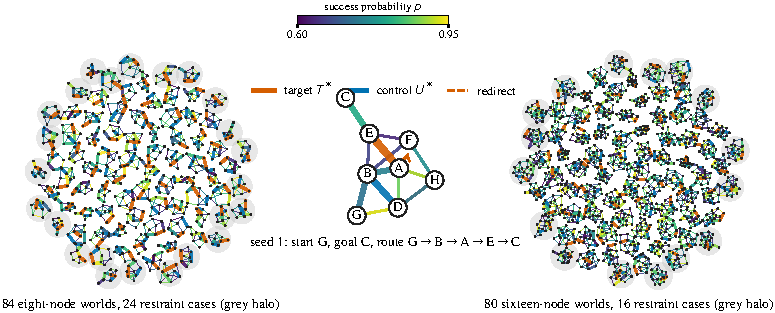
\includegraphics[width=\textwidth]{figures/fig_atlas.pdf}
\caption{All evaluated worlds and the running example.}
\label{fig:atlas}
\end{figure*}

\Cref{fig:atlas} shows every world we evaluate. The main family has eight nodes and six extra links. A larger, denser family has sixteen nodes and twenty. Seeds 1 to 30 were used in exploratory runs and are excluded from every confirmatory analysis. Of seeds 31 to 130, \nSeedsEight{} eight-node and \nSeedsSixteen{} sixteen-node worlds have an on-route link whose break keeps the goal reachable, and these form the run sets (\cref{app:method}). At the center is the running example, seed 1, with start G, goal C and optimal route G\,$\to$\,B\,$\to$\,A\,$\to$\,E\,$\to$\,C. Its target $\Tstar = \pa{A}{2}$ is the on-route link that the route-changing interventions edit, redirect sends the same action to F, and its off-route control is $\Ustar = \pa{D}{2}$.

\paragraph{Interventions.}
Each instance is a pair of worlds, $M_0$ and $M_1$, differing by at most one edit, which makes localization well defined. The route-changing scenarios all edit the same target link $\Tstar$, drawn from the best route so that the goal stays reachable. A difference in performance therefore reflects the kind of change rather than which link is hit. \Cref{tab:interventions} lists the six scenarios. Five edit a link and one edits nothing, and only redirect changes a destination. Degradation exists only in the stochastic mode, because a deterministic world admits only links that always or never work.

\begin{table}[!htb]
\centering
\small
\caption{Intervention scenarios.}
\label{tab:interventions}
\begin{tabularx}{\linewidth}{@{}l >{\raggedright\arraybackslash}X >{\raggedright\arraybackslash}X@{}}
\toprule
Scenario & Intervention & What it tests \\
\midrule
No change & none & false positives \\
Irrelevant & $\Ustar$ to $p = 0$ & change noticed, judged harmless \\
Silent break & $\Tstar$ to $p = 0$, still on the menu & inferring failure from absent successes \\
Hard removal & $\Tstar$ leaves the menu & control, visible by menu difference \\
Redirect & $\Tstar$ keeps $p$, new destination & destinations learned, or only rates? \\
Degradation & $\Tstar$ probability halved & re-planning after a partial change \\
\bottomrule
\end{tabularx}
\end{table}
Silent break and hard removal are the same event with and without a structural clue, so the gap between their scores shows how much performance comes from reading evidence rather than comparing menus. Hard removal can be solved from the menus alone and serves as a positive control.

Redirect keeps every success rate and moves only a destination. The action keeps its label at the new destination, so the menu is identical across periods and the change cannot be read from it. The irrelevant control sets an off-route link $\Ustar$ to $p = 0$ (\cref{app:families}). Irrelevant and silent break thus differ only in relevance.

\paragraph{What separates the two worlds.}
The design follows the evaluation framework of \citet{vafa2024}, with their automaton replaced by a Markov decision process because the outcome of an action here may be random. Each observation is a triple $x = (u, a, v')$, recording that action $a$ was attempted at node $u$ and that the packet then stood at node $v'$. Each period log is a sequence of such triples. Writing $P_{M}(v' \mid u, a)$ for the probability that world $M$ produces next node $v'$, the node-action pairs that separate the two worlds form the set
\begin{equation}
  \mathcal{D} = \{ (u, a) : P_{M_0}(\cdot \mid u, a) \neq P_{M_1}(\cdot \mid u, a) \} \cup \mathcal{R} ,
  \label{eq:D}
\end{equation}
where $\mathcal{R}$ holds the pairs on the menu of only one period. By construction $\mathcal{D}$ holds at most one pair. It is $\{\Tstar\}$ under the four route-changing interventions, $\{\Ustar\}$ under the irrelevant control, and none under no change. Every observation outside $\mathcal{D}$ is equally likely in both periods, so only observations at that pair can separate $M_0$ from $M_1$.

The probes follow from this reading. Detection and Localization ask whether the model notices that the two logs come from different worlds and whether it places the difference at the one pair in $\mathcal{D}$. Preservation asks whether pairs outside $\mathcal{D}$ keep the beliefs the model formed in Period A. The no change condition asks the same of the whole log. Route-taking can succeed without the distinction being drawn, so crossing Localization with route optimality separates knowing where the world changed from acting well after it changed.
% ===== end sections/03_environment.tex =====

% ===== begin sections/04_evidence_probes_baselines.tex =====
\section{Evidence, probes and baselines}\label{sec:probes}
\paragraph{Evidence.}
The model never sees the graph. It sees a log of attempts and outcomes in two blocks, Period A from before the intervention and Period B from after, plus the action menu at each node. $K$ is the minimum number of times each link (node-action pair) is attempted in each period. For example, $K = 5$ means that every link is attempted at least five times, and the prompt shows five attempts for every link. We collect the evidence with a fixed policy that does no reasoning, separately in each world, attempting the least-tried action at each node until every listed pair has at least $K$ attempts (\cref{app:evidence}).

A silently broken link stays on the menu, so it too receives at least $K$ attempts in Period B, all of them failures, which is exactly the detection evidence.

In the main runs each record is a bare triple [current node, action, observed next node], pooled and shuffled, so that order carries no information and each line is an atomic fact. The prompt states the rules of the world and defines a success probability as the fraction of visible observations that end at a different node (\cref{app:prompts}). It therefore already asks the model to count. The minimal-logs contrast removes these instructions. The rules also ask the model to keep the most recent destination of an action that has no successful observation in the current period. Because this could pull a silently broken link into the plan, we also run a variant without it (\cref{sec:setup}).

\paragraph{Two-turn protocol.}
The model first sees only Period A and gives its best route and its beliefs about five selected pairs, each stating whether the action is available, its destination and its success probability. Period B is then added to the same conversation, and a single answer reports whether anything changed, which pair changed, the same five beliefs with a changed or unchanged label for each, a belief about every other listed pair, and the best route now.

Localization is read from a free answer over every pair on the menu (\cref{app:twoturn}). Preservation asks whether the model kept its Period A beliefs about the queried unchanged links and labeled them unchanged, so it shares no pair with Localization. Committing the model to a Period A route and beliefs before Period B appears makes updating measurable against its own earlier answers.

\paragraph{Single-turn setting.}
In the Single-turn setting one fresh call shows both periods at once and asks for the same Period B answer, so the difference from the two-turn protocol measures how much apparent updating was really planning from Period B (\cref{app:singleturn}).

\paragraph{Scoring.}
We request every answer as exactly one JSON object with a fixed shape. An answer that still does not parse after one repair request counts as incorrect on every probe it should have answered, so models and references are compared on identical instances (\cref{sec-scoring}). Results excluding unparsed instances are secondary. Detection is reported as sensitivity, the share of changed instances reported as changed, and specificity, the share of no change instances reported as unchanged. Localization requires the exact pair. A model that reports no change has not localized, and Localization conditional on a reported change is a secondary measure.

We count a stated probability as correct within a tolerance $\tau$ fixed before the main runs: $\tau = 0.15$ in the stochastic mode and $\tau = 0$ (an exact match) in the deterministic mode. For Preservation, the stated probability of an unchanged pair must instead stay within the 95 percent sampling-noise band of its Period A statement (\cref{sec-scoring}).

We check routes in the true simulator, never by the model's own account. The grader walks the route, computes its expected cost $C(r)$ by \cref{eq:cost} and its regret
\begin{equation}
  \mathrm{regret}(r) = C(r) - \min_{r'} C(r') ,
  \label{eq:regret}
\end{equation}
and counts any valid route with zero regret as optimal, whether or not it equals the canonical oracle route. Because the Period B answer states a belief about every listed pair, a route is also checked against the model's own beliefs. It is \emph{self-consistent} if it uses no action the model states is unavailable or has $\hat{p} \le 0.05$, and is optimal under the stated destinations and probabilities. A route through a broken link gets its own failure status, silent broken edge, with infinite expected cost. The primary routing measure is the optimal-route rate over all instances, so an invalid route counts as not optimal. The secondary measure is median regret with invalid routes at $+\infty$.

\subsection{Evidence-only reference detectors}\label{sec:baselines}
Evidence-only references answer the same four probes by arithmetic over the same prompt view, at the same rendering and per-pair budget, with no reasoning. They range from two counting heuristics, the \emph{rate counter} and the \emph{transition counter}, through an uninformative \emph{Bayesian observer} to a \emph{generator-aware observer} that also knows the generator's priors but not its target rule. The last is close to, but not exactly, an ideal observer, and it is the reference against which we measure the gap. All four route by Dijkstra's algorithm on the observed Period B rates and destinations, and Detection thresholds are calibrated on held-out seeds at a false-alarm rate of at most 10 percent (\cref{app:refdetectors}).

What a reference reads decides what it can see. From success rates alone a redirect looks like no change: \redirNbNoChangeRate{} percent of a redirect instance's nearest neighbors are no change instances, against \redirNbNoChangeTrans{} percent from full outcome distributions (\cref{fig:evidence} in \cref{app:refdetectors}).

\begin{figure}[!htb]
\centering
\begin{tikzpicture}
\begin{axis}[
    width=0.93\linewidth, height=4.6cm, xmin=-0.02, xmax=1.02, ymin=0.5, ymax=6.5,
    ytick={1,...,6}, yticklabels={Degr.\ (restraint),Degr.\ (moves),Redirect,Hard removal,Silent break,Irrelevant},
    xtick={0,0.25,0.5,0.75,1}, xticklabel style={/pgf/number format/fixed, /pgf/number format/precision=2},
    xlabel={Localization at $K = 10$},
    axis lines=left, tick style={draw=ecMuted}, axis line style={draw=ecMuted},
    label style={font=\small}, tick label style={font=\scriptsize},
    xmajorgrids, grid style={draw=ecLine!50, line width=0.3pt},
    legend columns=4, legend style={font=\scriptsize, draw=none, fill=none, at={(0.5,1.02)}, anchor=south, column sep=3pt},
    every axis plot/.append style={only marks, mark size=1.8pt, error bars/x dir=both, error bars/x explicit, error bars/error bar style={line width=0.5pt}},
  ]
  \addplot[color=ecRefRate, mark=o] coordinates {\figRefRate};
  \addlegendentry{rate}
  \addplot[color=ecRefTrans, mark=triangle] coordinates {\figRefTrans};
  \addlegendentry{transition}
  \addplot[color=ecRefBayes, mark=triangle*] coordinates {\figRefBayes};
  \addlegendentry{Bayesian}
  \addplot[color=ecRefGen, mark=diamond*] coordinates {\figRefGen};
  \addlegendentry{generator-aware}
\end{axis}
\end{tikzpicture}
\caption{Localization by the four references, with 95\% intervals.}
\label{fig:refs}
\end{figure}

\Cref{fig:refs} shows Localization by each reference at $K = 10$. Colour marks what a reference reads: success rates, full outcome distributions, or also the generator's priors. Redirect is invisible to success rates (\locRateRedTen) and plain to every other reference, which makes it a manipulation check. \Cref{app:refdetectors} gives every $K$ and how often the reference route is optimal.

The references are the standard against which we read model results. Localization is read as a gap to the generator-aware observer at each $K$, and whether a gap reflects tallying or the use of evidence is addressed by the counts-given contrast. The references also enforce a rule: no model is said to fail at Localization on an instance that no reference can solve. $K$ is therefore not a nuisance parameter. It sets how much of the answer the logs contain, so it is an independent variable, and a result at a single $K$ is one point on a curve whose shape the references fix in advance.
% ===== end sections/04_evidence_probes_baselines.tex =====

% ===== begin sections/04b_agentic_exploration.tex =====
\section{Agentic exploration}\label{sec:agentic-exploration}
In the agentic arm the model collects its own evidence. Where the two-turn protocol gives it a log collected by a fixed policy (\cref{sec:probes}), here it chooses each action itself and so determines which information about the network becomes available.

\subsection{Exploration phases}\label{sec:agentic-phases}
The model first interacts with $M_0$ for $E_0$ episodes and then continues in $M_1$ for $E_1$ episodes. Under no change the two worlds are identical. Each episode is an attempt to reach $g$ from $s_{\mathrm{start}}$ within at most $H$ action attempts. The main runs use $E_0 = E_1 = 4$ and $H = 25$ (\cref{app:agentic}). The packet is reset at the start of each episode, while the interaction history is kept across episodes and phases. An episode ends when the goal is reached or the step budget is exhausted (\cref{app:interaction}).

The model is given the goal and asked to reach it in as few steps as possible. It is told that actions may fail, that link reliabilities may or may not change between episodes, and that nothing will announce such a change (\cref{app:prompts}). The topology, destinations and transition probabilities are not disclosed.

Before each action the model receives its current node, the available action labels, the remaining step budget and feedback about its previous attempt. The interaction is one growing conversation, so every choice is conditioned on the full history, and at the transition to $M_1$ the model is told only that it has been placed back at the start. The formal interaction model, the announced variant and the rule for unavailable actions are in \cref{app:interaction}.

\paragraph{Prompt conditions.}
We run the arm under three prompts. Under task\_only the model receives only the task. Under model\_first it also writes a free-text description of the network before every episode after the first, including the first episode in $M_1$. Under graph\_given it receives the current network, with every destination and success probability, at the start of each phase, so exploration is unnecessary and the condition serves as a ceiling. Comparing model\_first with task\_only asks whether stating a model of the world changes the actions taken in it (H6).

\subsection{Behavioral and explicit evaluation}\label{sec:agentic-eval}
Behavior is scored separately in $M_0$ and $M_1$ by goal success, steps to goal, optimal action rate, route regret, use of the changed action and the switch away from it, and agreement with a reference reconstructed only from the model's own $M_0$ observations (\cref{app:agentic}). After exploration, the model answers the same four probes as in the two-turn protocol, each presented independently on a copy of the completed transcript, so no probe sees the answer to another. The answers are scored by the rules of \cref{sec:probes}, and comparing them with the model's choices shows whether what it reports about the world agrees with what it did.
% ===== end sections/04b_agentic_exploration.tex =====

% ===== begin sections/05_setup.tex =====
\section{Experimental setup}\label{sec:setup}
\paragraph{Models.}
We evaluate five models chosen to span tiers and providers rather than to be ranked: Gemma 4 E4B~\cite{gemma4}, a small open model run locally. GPT-4o~\cite{openai2024gpt4o}, a previous-generation model. GPT-5.6 Sol~\cite{gpt56sol}, a current reasoning model. DeepSeek V4 Flash~\cite{deepseekv4flash}, an open-weight mixture-of-experts model, and Kimi K2.7 Code~\cite{kimik27}, an open-weight coding model from a third provider. Every model sees identical prompts through the same harness. We request every model by its exact dated version (\cref{tab:models}).

\paragraph{Runs.}
All confirmatory runs use seeds 31 to 130. \Cref{app:runs} lists the conditions, settings and budgets $K$ that each model runs. The agentic arm runs on the first \nAgentic{} confirmatory seeds with stochastic silent break (\cref{sec:res-agentic}). Each instance is answered once, at temperature 0 where the provider allows it. GPT-5.6 Sol and Kimi K2.7 Code reason by default and run at their providers' settings (\cref{tab:models}).

\begin{table}[!htb]
\centering
\scriptsize
\caption{Hypotheses.}
\label{tab:hyp}
\begin{tabularx}{\linewidth}{@{}l >{\raggedright\arraybackslash}X >{\raggedright\arraybackslash}X@{}}
\toprule
& Quantity & Prediction \\
\midrule
H1 & silent break, no keep-destination rule: share of Period B routes through the broken link when the model's own belief gives it $\hat{p} \le 0.05$ & lower bound above 0.10 \\
H2 & silent break Localization, counts given $-$ core & above 0 \\
H3 & silent break optimal-route rate, Single-turn $-$ two-turn & above 0 \\
H4 & agentic, all runs: share of choices of the broken link made after six consecutive observed failures of it & lower bound above 0.10 \\
H5 & silent break Localization, $K = 20$ $-$ $K = 5$ & above 0 \\
H6 & agentic, silent break: H4's share under model\_first $-$ under task\_only & below 0 \\
\bottomrule
\end{tabularx}
\end{table}
\paragraph{Hypotheses and analysis.}
\Cref{tab:hyp} lists the hypotheses. All are one-sided, use the stochastic eight-node family, and form one family each across the five models. We fixed the analysis plan before the confirmatory runs and revised it three times before any confirmatory data existed. The conditions of each hypothesis are in \cref{app:hypconditions}, and rules, power and revisions in \cref{app:method,app:pilots}.

\begin{table*}[t]
\centering
\small
\setlength{\tabcolsep}{3pt}
\caption{Core results, stochastic mode, $K = 10$.}
\label{tab:main}
\adjustbox{max width=\linewidth}{% ===== begin tables/main_results.tex =====
% Generated by scripts/make_tables.py. Do not edit by hand.
\begin{tabular}{@{}l cccc cccc cccc cccc cccc cccc@{}}
\toprule
& \multicolumn{4}{c}{References} & \multicolumn{4}{c}{Gemma 4 E4B} & \multicolumn{4}{c}{GPT-4o} & \multicolumn{4}{c}{GPT-5.6 Sol} & \multicolumn{4}{c}{DeepSeek V4 Flash} & \multicolumn{4}{c}{Kimi K2.7 Code} \\
\cmidrule(lr){2-5} \cmidrule(lr){6-9} \cmidrule(lr){10-13} \cmidrule(lr){14-17} \cmidrule(lr){18-21} \cmidrule(lr){22-25}
Condition & Rate & Bayes & Gen. & Route & Det & Loc & Pres & Route & Det & Loc & Pres & Route & Det & Loc & Pres & Route & Det & Loc & Pres & Route & Det & Loc & Pres & Route \\
\midrule
No change & -- & -- & -- & 0.76 & \RES & -- & \RES & \RES & \RES & -- & \RES & \RES & \RES & -- & \RES & \RES & \RES & -- & \RES & \RES & \RES & -- & \RES & \RES \\
Irrelevant & 0.99 & 0.99 & 1.00 & 0.79 & \RES & \RES & \RES & \RES & \RES & \RES & \RES & \RES & \RES & \RES & \RES & \RES & \RES & \RES & \RES & \RES & \RES & \RES & \RES & \RES \\
Silent break & 0.93 & 0.95 & 1.00 & 0.86 & \RES & \RES & \RES & \RES & \RES & \RES & \RES & \RES & \RES & \RES & \RES & \RES & \RES & \RES & \RES & \RES & \RES & \RES & \RES & \RES \\
Hard removal & 1.00 & 1.00 & 1.00 & 0.82 & \RES & \RES & \RES & \RES & \RES & \RES & \RES & \RES & \RES & \RES & \RES & \RES & \RES & \RES & \RES & \RES & \RES & \RES & \RES & \RES \\
Redirect & 0.08 & 1.00 & 1.00 & 0.83 & \RES & \RES & \RES & \RES & \RES & \RES & \RES & \RES & \RES & \RES & \RES & \RES & \RES & \RES & \RES & \RES & \RES & \RES & \RES & \RES \\
Degr.\ (moves) & 0.50 & 0.45 & 0.67 & 0.62 & \RES & \RES & \RES & \RES & \RES & \RES & \RES & \RES & \RES & \RES & \RES & \RES & \RES & \RES & \RES & \RES & \RES & \RES & \RES & \RES \\
Degr.\ (restraint) & 0.54 & 0.54 & 0.62 & 0.50 & \RES & \RES & \RES & \RES & \RES & \RES & \RES & \RES & \RES & \RES & \RES & \RES & \RES & \RES & \RES & \RES & \RES & \RES & \RES & \RES \\
\midrule
Parse failures & & & & & & & \RES & & & & \RES & & & & \RES & & & & \RES & & & & \RES & \\
\bottomrule
\end{tabular}
% ===== end tables/main_results.tex =====
}
\end{table*}
\begin{table}[!htb]
\centering
\scriptsize
\setlength{\tabcolsep}{3pt}
\caption{Hypothesis results.}
\label{tab:verdicts}
\adjustbox{max width=\linewidth}{% ===== begin tables/verdicts_compact.tex =====
% Generated by scripts/make_tables.py. Do not edit by hand.
\begin{tabular}{@{}l ccccc@{}}
\toprule
Hyp. & Gemma 4 E4B & GPT-4o & GPT-5.6 Sol & DeepSeek V4 Flash & Kimi K2.7 Code \\
\midrule
H1 & \RES & \RES & \RES & \RES & \RES \\
H2 & \RES & \RES & \RES & \RES & \RES \\
H3 & \RES & \RES & \RES & \RES & \RES \\
H4 & \RES & \RES & \RES & \RES & \RES \\
H5 & \RES & \RES & \RES & \RES & \RES \\
H6 & \RES & \RES & \RES & \RES & \RES \\
\bottomrule
\end{tabular}
% ===== end tables/verdicts_compact.tex =====
}
\end{table}
% ===== end sections/05_setup.tex =====

% ===== begin sections/06_results.tex =====
\section{Results}\label{sec:results}

% Every number in this section comes from tables/ and figures/*_data.tex,
% which scripts/make_tables.py writes from the run artifacts. Write the
% prose last, and give every cell cited in a sentence its n.

\Cref{tab:main} reports the stochastic eight-node family at $K = 10$, with one row per condition. Det is the share of instances the model reported as changed, which in the no change row is the false-alarm share. Loc is the share of seeds on which the model named the exact changed pair. Pres is the mean Preservation over the four or five queried pairs that did not change. Route is the share of all instances whose Period B route is optimal. For comparison, the table gives the Localization of three references and the optimal-route rate of the reference route. The last row gives each model's parse-failure rate. Each cell covers \nSeedsEight{} seeds. Degradation has two rows, the \nDegMove{} seeds on which the best route moves and the \nDegRestraint{} restraint cases on which it does not. Degradation is underdetermined at $K = 10$ (\cref{sec:baselines}), so these cells are descriptive only.

\Cref{tab:verdicts} gives each hypothesis per model as an estimate and a symbol. $\uparrow$ means the estimate clears its threshold after correction across models, and $\sim$ means it does not. A dagger marks fewer than 10 qualifying instances. \Cref{app:full} gives the full intervals, the sixteen-node family, the deterministic mode, Detection and the remaining contrasts.

\subsection{Gap to the observer}\label{sec:res-evidence}
\Cref{tab:gap} in \cref{app:full} gives, for silent break, the difference between each model's Localization and the generator-aware observer's on the same seeds at each $K$, with its 95\% interval. On silent break the gap to the generator-aware observer is \RES{} at $K = 5$, \RES{} at $K = 10$ and \RES{} at $K = 20$. H5, that Localization rises from $K = 5$ to $K = 20$, holds for \RES{} of the five models. On redirect, the manipulation check, models localize \RES{} of seeds, against \pctGenRedMin{} percent or more for the generator-aware observer. Without the counting instructions, silent-break Localization changes by \RES.

\subsection{Tabulation and use of evidence}\label{sec:res-counts}
With the counts given, silent-break Localization changes by \RES{} on average, and H2 holds for \RES{} of the five models.. A rise would show that tabulation helps. Because the tabulated view also changes format and length, it would not by itself show that failures are tallying failures, and a null result would license no conclusion.

\subsection{Report and plan}\label{sec:res-belief}
\Cref{tab:belief} in \cref{app:full} crosses, for stochastic silent break at $K = 10$, whether the model's own Period B belief gives the broken link $\hat{p} \le 0.05$ with whether its Period B route uses that link, one instance per seed, for the prompt without and with the keep-destination rule. Without the keep-destination rule, \RES{} of the instances in which a model states that the broken link no longer works still route through it, and H1 holds for \RES{} of the five models. Among instances that state the link usable, the share is \RES. Of all Period B routes, \RES{} are self-consistent.

\subsection{Report and action}\label{sec:res-agentic}
In the agentic arm the model chooses the actions itself. After six consecutive observed failures of the broken link, models still choose it in \RES{} of such choices over all runs and in \RES{} over runs that localize the break, and H4 holds for \RES{} of the five models. The adaptation lag is \RES{} steps, against a median of \lagRefAgent{} for the evidence-only reference agent (\nLagRefAgent{} of \nLagRefSeeds{} seeds, where it tried the broken link). Under model\_first the share is \RES, a difference of \RES{} from task\_only, and H6 holds for \RES{} of the five models. Under graph\_given it is \RES. The protocol is described in \cref{sec:agentic-exploration}, with details in \cref{app:agentic}.

\subsection{Commitment and route choice}\label{sec:res-commit}
Shown both periods at once, models reach the optimal silent-break route \RES{} more often than in the two-turn protocol, and H3 holds for \RES{} of the five models.
% ===== end sections/06_results.tex =====

% ===== begin sections/07_discussion.tex =====
\section{Discussion}\label{sec:discussion}
Reading every model answer against evidence-only references changes what a failure means. A model that misses a change the logs make visible has failed. A model that misses a change no reference can find has not, and without the references the two cannot be told apart. Tabulating the counts \RES{} the gap to the observer (H2). Models that report a break avoid it in \RES{} of their plans (H1) and in \RES{} of their actions after repeated failures (H4).

\Cref{app:future} lists the directions left open, including a finetuning arm.
% ===== end sections/07_discussion.tex =====

% ===== begin sections/08_limitations.tex =====
\section*{Limitations}
The largest limit cannot be lifted within this study. The work uses two graph families from one generator, eight and sixteen nodes, with at most one edit per instance, and the world reaches the model only as logs of attempts. It is a demonstration on a constructed environment rather than a measurement of model behavior in general. Nothing in it is specific to language, and the same probes and references must be run on a world described in natural language, such as a text game or a tool interface, before its conclusions carry over. The probes measure agreement between report, plan and action, not the coherence of a recovered map~\cite{vafa2024}.

The prompt defines success probability as a fraction of observations, so part of any agreement with the references is instruction-following. The minimal-logs contrast measures how much. The strongest reference is not an exact ideal observer, since it does not model the generator's rule for choosing targets. We report no human baseline. The references bound what the logs allow, but they do not show how people would read the same logs. In the two-turn protocol the report and the plan are fields of one answer, so H1 measures report-plan consistency, and only the agentic arm measures action. That arm covers silent break on \nAgentic{} seeds.

The \nSeedsEight{} seeds detect differences of roughly \mdePaired{} after correction across models. Smaller differences cannot be distinguished from none, and no ranking of models is attempted. Five models span several tiers and providers but not the space of models. The four accessed through commercial interfaces may change without notice, which pinned versions and access dates only partly address, and two of them reason by default and run at their providers' settings rather than at temperature 0. In the deterministic mode \nDetTies{} of \nSeedsEight{} seeds have tied optimal routes, so deterministic routing is descriptive. The analysis plan was fixed before the confirmatory runs and revised three times before any confirmatory data existed, but it was not registered in a public registry.

\section*{Ethics statement}
The study uses synthetic graphs and no human data. Model access was through public APIs and a locally run open model. All code and run artifacts are public~\cite{ecpm2026}. AI assistants (Claude and ChatGPT) were used extensively throughout the project, including for writing, coding, analysis and figures. The authors reviewed all of it and take responsibility for the content.
% ===== end sections/08_limitations.tex =====






% Line numbers paused for the reference list: lineno misplaces them inside it in two-column mode.
\nolinenumbers
\bibliography{references}

% ####################################################################
% #                            APPENDIX                              #
% #  Same PDF, after the references; not counted in the page limit.  #
% #  Reviewers are not required to read it, so the main paper must   #
% #  stand on its own.                                               #
% ####################################################################
\onecolumn
\linenumbers
\appendix
% ===== begin sections/appendix_a_methodology.tex =====
\section{Experimental details}\label{app:method}

\subsection{Formal definition, continued}\label{app:formal}
This continues the formal definition of \cref{sec:environment}.
A successful attempt moves the packet to the action's
destination, whereas an unsuccessful attempt leaves it at
the current node. Each attempt incurs a cost of one:
\[
c(s,a)=1
\qquad\text{for }s\neq g.
\]
Conditional on the selected node-action pair, outcomes are
sampled using its fixed success probability. Transition
probabilities remain constant within each environment.

The routing objective is to minimize the expected number
of attempts required to reach the goal:
\begin{align*}
V_w^*(s)
&=
\inf_{\pi}
\mathbb{E}_{M_w,\pi}
\left[
N_g \mid s_0=s
\right],\\
N_g&=\inf\{t\geq 0:s_t=g\}.
\end{align*}
Here $\pi$ denotes a routing policy, and
$N_g=+\infty$ if the goal is never reached.

\subsection{Graph generation, families and modes}\label{app:families}
\paragraph{Graph generation.}
A fixed generator builds each graph. It places the eight nodes in a random order and chains them toward the goal, which guarantees that every node can reach it. Six further random links then add alternative routes, and every node except the goal receives at least two outgoing links, so that breaking one link usually leaves an alternative. Seeds where no on-route link can break without cutting off the goal are excluded (below). Each link receives a success probability $p$. Because a failed attempt leaves the packet in place, crossing a link with probability $p$ takes $1/p$ attempts on average, and the expected cost of a route $r = (v_0, v_1, \dots, v_n)$ is
given by \cref{eq:cost}.
The optimal route is therefore a shortest path under edge weights $1/p$, which Dijkstra's algorithm~\cite{dijkstra1959} finds exactly, so every reference answer is computed without training any policy. The goal is the last node of the chain, and the start node is the node farthest from the goal in hop count.

A seed is the integer that builds a graph, and reusing it rebuilds that world exactly. \Cref{fig:seed1} shows seed 1, the running example, with start G, goal C and sixteen links. Route links are labeled by action and success probability. The thick dark path is the optimal route G\,$\to$\,B\,$\to$\,A\,$\to$\,E\,$\to$\,C. The orange link is the target $\Tstar = \pa{A}{2}$ edited by the route-changing interventions, and the dashed orange arrow shows where redirect sends the same action. The blue link is the off-route control $\Ustar = \pa{D}{2}$. In the deterministic mode every probability is 1 and the layout is identical.

\Cref{fig:seed1} draws the running example in full, and \cref{fig:atlaslarge} repeats the atlas of \cref{fig:atlas} at full size. Each world is drawn with its own force-directed layout. Positions and distances between worlds carry no meaning.

\begin{figure*}[t]
\centering
\scalebox{0.70}{%
\begin{tikzpicture}[
    x=1cm, y=1cm, >={Stealth[length=2.2mm,width=1.6mm]},
    node/.style={circle, draw=ecRoute, line width=0.6pt, fill=white, minimum size=8.5mm, inner sep=0pt, font=\small\rmfamily},
    term/.style={node, line width=1.2pt},
    lab/.style={font=\scriptsize\rmfamily, fill=white, inner sep=1.2pt, text=ecRoute},
    link/.style={->, draw=ecMuted, line width=0.6pt},
    route/.style={->, draw=ecRoute, line width=1.3pt},
  ]
  \node[term] (G) at (0,0) {G};
  \node[node] (B) at (3,0) {B};
  \node[node] (A) at (6,0) {A};
  \node[node] (E) at (9,0) {E};
  \node[term] (C) at (12,0) {C};
  \node[node] (D) at (1.5,-3.2) {D};
  \node[node] (H) at (4.5,-3.2) {H};
  \node[node] (F) at (7.5,-3.2) {F};
  \node[font=\scriptsize\rmfamily, text=ecMuted, above=1mm of G] {start};
  \node[font=\scriptsize\rmfamily, text=ecMuted, above=1mm of C] {goal};
  \draw[route] (G) -- node[lab, above=1pt] {$a_2$ 0.73} (B);
  \draw[route] (B) -- node[lab, above=1pt] {$a_1$ 0.75} (A);
  \draw[->, draw=ecTarget, line width=2.2pt] (A) -- node[lab, above=1pt, text=ecTarget] {$\Tstar$ $a_2$ 0.74} (E);
  \draw[route] (E) -- node[lab, above=1pt] {$a_2$ 0.81} (C);
  \draw[link] (E) to[out=150, in=30, looseness=0.9] (B);
  \draw[link] (G) to[bend right=14] (D);
  \draw[link] (D) to[bend right=14] (G);
  \draw[->, draw=ecControl, line width=1.6pt] (D) -- node[lab, right=1pt, pos=0.5, text=ecControl] {$\Ustar$ $a_2$ 0.92} (B);
  \draw[link] (D) to[bend left=12] (H);
  \draw[link] (H) to[bend left=12] (D);
  \draw[link] (H) to[bend left=14] (A);
  \draw[link] (A) to[bend left=14] (H);
  \draw[link] (A) -- (D);
  \draw[link] (B) -- (F);
  \draw[link] (F) -- (E);
  \draw[link] (F) -- (H);
  \draw[->, draw=ecTarget, line width=0.9pt, dashed] (A) to[bend left=10] node[lab, pos=0.62, text=ecTarget, right=1pt] {redirect} (F);
\end{tikzpicture}}
\caption{Seed 1, stochastic mode.}
\label{fig:seed1}
\end{figure*}
\begin{figure*}[p]
\centering
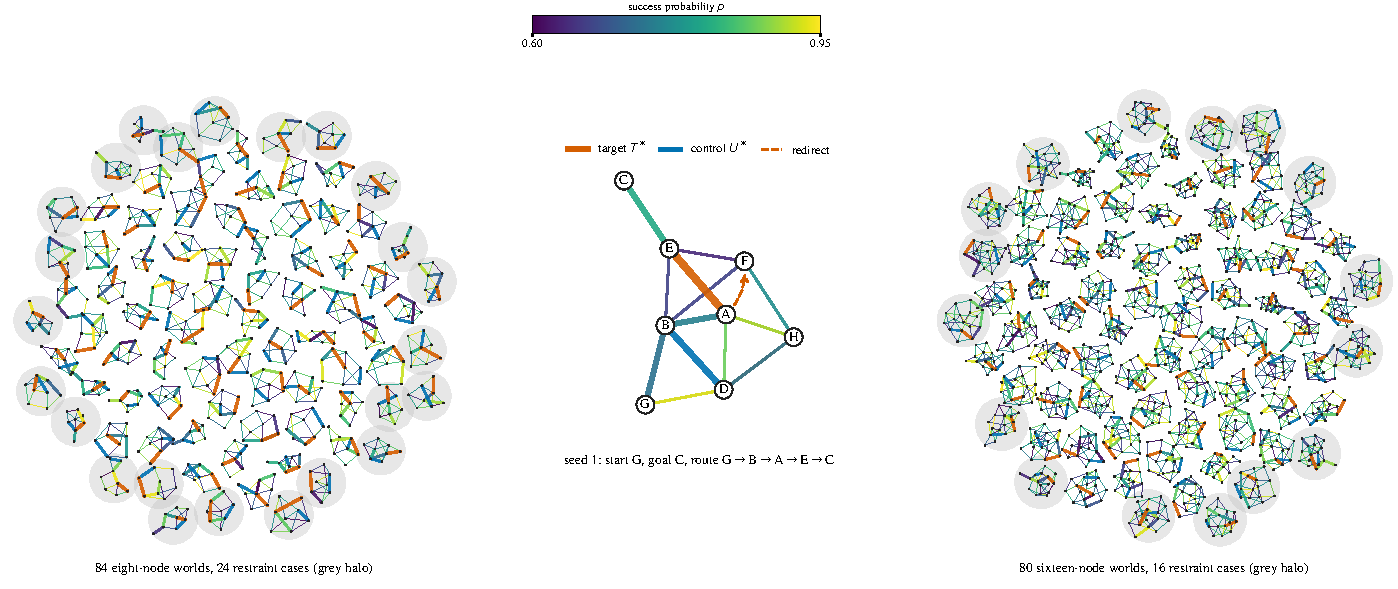
\includegraphics[width=\textwidth]{figures/fig_atlas_large.pdf}
\caption{World atlas at full size.}
\label{fig:atlaslarge}
\end{figure*}

\paragraph{Graph families.}
The generator takes the number of nodes and of extra links as parameters. The main family has eight nodes and six extra links. A second, larger and denser family has sixteen nodes and twenty extra links, which lengthens routes and multiplies alternatives. Both come from the same generator, so a structurally different family remains future work.

\paragraph{Deterministic and stochastic modes.}
The main results use the stochastic mode. The deterministic mode serves as an exact-counting check and is reported in \cref{app:full}. In the deterministic mode every link works, so $p = 1$, and cost is hop count. In the stochastic mode link probabilities are drawn uniformly from 0.60 to 0.95 and rounded to two decimals, so every link fails sometimes and none so often that it could be mistaken for a missing link. The deterministic mode is logical inference, since one failure proves a break, while the stochastic mode is statistical inference from a sample. Generation runs in a matched mode, so the deterministic and stochastic instances of a seed share the start, the goal and the intervention target. A comparison between the modes therefore changes only the probabilities.

\subsection{Single-turn setting}\label{app:singleturn}
In the Single-turn setting one fresh call shows both periods at once and asks for the same Period B answer. A model shown both periods at once can route around a break it never noticed, so Single-turn results measure planning from evidence rather than updating. Single-turn is kept as a comparison condition on the same seeds and the same $K$, so the difference between the two settings measures how much apparent updating was really planning from Period B.

\subsection{Queried pairs}\label{app:twoturn}
The target is among the five on half of the seeds, decided by seed alone so that every condition of a seed sees the same set, except that under irrelevant the irrelevant link takes the target's place. Otherwise all five are unchanged links. Localization is read from a free answer over every pair on the menu, so the queried set does not narrow the candidates.

The irrelevant control draws $\Ustar$ from the links on no optimal route, ties included, so the best route and its uniqueness are preserved, and sets it to $p = 0$ in both modes.

\subsection{Seed eligibility}
A seed qualifies for a condition if (1) the goal stays reachable under the scenario, (2) a control leaves the best route untouched while a route-changing scenario moves it, and (3) the best route is unique before and after the edit, since under a tie a correct re-plan is indistinguishable from a lucky choice. The second criterion is applied per condition. Seeds that fail it only because halving the target makes no detour cheaper are kept as restraint cases, because the edit is real and detectable, so Detection, Localization and Preservation remain informative, while Route-taking there is scored as a restraint check, since the pre-change route is still optimal. Under degradation the route moves on \nDegMove{} of the \nSeedsEight{} eight-node seeds, and the other \nDegRestraint{} are restraint cases. The seed list is generated from these criteria rather than written by hand, and the run set is the intersection over conditions, so every condition is compared on the same graphs. Seeds 1 to 30 were used in exploratory runs and are excluded. \Cref{tab-seeds} gives the counts over seeds 31 to 130 in the stochastic mode. In the deterministic mode integer hop costs create ties on \nDetTies{} of the \nSeedsEight{} eight-node seeds, so uniqueness is relaxed there on the same seeds and deterministic Route-taking is reported descriptively and enters no hypothesis.

\begin{table}[!htb]
\centering
\scriptsize
\caption{Eligible seeds, 31 to 130.}
\label{tab-seeds}
\begin{tabular}{@{}l cc cc@{}}
\toprule
& \multicolumn{2}{c}{8 nodes} & \multicolumn{2}{c}{16 nodes} \\
\cmidrule(lr){2-3} \cmidrule(lr){4-5}
Condition & eligible & restraint & eligible & restraint \\
\midrule
Silent break & 84 & 0 & 80 & 0 \\
Hard removal & 84 & 0 & 80 & 0 \\
Redirect & 84 & 0 & 80 & 0 \\
Degradation & 60 & 24 & 64 & 16 \\
Irrelevant & 100 & 0 & 100 & 0 \\
No change & 100 & 0 & 100 & 0 \\
\bottomrule
\end{tabular}
\end{table}

\Cref{tab-seeds} lists, per condition and family, the seeds on which the route-changing scenario moves the route or the control leaves it, and the restraint cases. The run set is the \nSeedsEight{} eight-node and \nSeedsSixteen{} sixteen-node seeds eligible for silent break. No change and irrelevant build on further seeds that are not used, so that every condition is compared on the same graphs.


\subsection{Scoring}\label{sec-scoring}
The parser reads the first balanced JSON object that parses, ignoring surrounding prose and code fences, and the one repair request is worded the same for every model.


Preservation is defined in \cref{sec:probes}. Its noise band replaces a fixed tolerance in the stochastic mode, and the fixed tolerance $\tau$ is used only for belief accuracy, which is reported in \cref{tab:beliefacc}.

For Preservation a fixed tolerance would penalize faithful reporting in the stochastic mode, since sampling noise alone moves the observed rate of a healthy link by more than $\tau$ on \pctOverTau{} percent of healthy pairs of held-out seeds at $K = 10$. The stated probability of an unchanged pair must therefore stay within the 95 percent noise band of its Period A statement, $1.96\sqrt{2\bar{p}(1-\bar{p})/K}$ with $\bar{p}$ the mean of the two statements, which the observed rates of healthy links exceed on \pctOverBand{} percent of those pairs.

A route using a broken link gets its own failure status, silent broken edge, with infinite expected cost. This can happen even when the model correctly reports the break. A route that uses an action missing from the menu, for example after a hard removal, is an illegal action. Format problems are separate. Overshoot occurs when the goal node is passed and the model continues to another node, and truncation covers answers cut off before the object closes. Both are recorded as parse or walk failures rather than as routing errors.



\paragraph{Reference detectors.}\label{app:refdetectors}
An evidence-only baseline answers the same four probes by arithmetic over the same prompt view, with no reasoning. It sees exactly what the model sees, at the same rendering and the same per-pair budget. For Detection it reports a change when a pair leaves the menu or when the largest change in observed success rate between the periods clears a threshold. For Localization it names the pair with the largest change, and a menu removal wins outright. For Preservation it marks exactly the localized pair as changed. For Route-taking it runs Dijkstra's algorithm on the observed Period B rates and destinations, with weight $1/\hat{p}$ per hop. We call it the \emph{rate counter}. The \emph{transition counter} and the uninformative \emph{Bayesian observer} (\cref{app:method}) compare full outcome distributions instead of rates. The \emph{generator-aware observer} also knows how the worlds are made: success probabilities are uniform on $[0.60, 0.95]$, at most one pair changes, and a change sets $p$ to zero, halves it, or moves the destination. It computes the posterior over no change and each pair and localizes the most probable pair. It does not model which links the generator may target, so it is close to, but not exactly, an ideal observer. It is the reference against which the gap is measured. All four route identically, by Dijkstra's algorithm on the observed Period B rates and destinations, and this reference route is scored like a model's. Because the queried set could still hint at the target, the references are also reported restricted to the queried pairs (\cref{app:full}). Detection thresholds are set per $K$ on \nHeldEight{} held-out seeds (1000 to 1099, same eligibility filter and matched generation) at a false-alarm rate of at most 10 percent. At $K = 10$ the Bayesian observer then detects \pctBayesDetSB{} percent of held-out silent breaks and the rate counter \pctRateDetSB{} percent (\cref{tab:calibration}).

\paragraph{References.}\label{sec-baseline}
All references answer by arithmetic over the prompt view and refuse to run if handed any evaluator-only field. They differ only in Detection and Localization. The rate counter scores each pair by the change in observed success rate, the transition counter by the total-variation distance between the two periods' outcome distributions, and the Bayesian observer by the log Bayes factor of separate against shared Dirichlet-multinomial outcome distributions (uniform prior, $\alpha = 1$). The generator-aware observer computes the posterior over no change and each pair under the generator's prior: $p$ uniform on $[0.60, 0.95]$ (integrated on a 400-point grid), the six scenarios equally likely, a change of the zero, halving or redirect type, and every pair equally likely to be the target. Hard removal is read from the menus. On the \nSeedsEight{} eight-node seeds it localizes silent break on \locGenSBFive, \locGenSBTen{} and \locGenSBTwenty{} of seeds at $K = 5$, 10 and 20, degradation on \locGenDegFive, \locGenDegTen{} and \locGenDegTwenty, and redirect on \locGenRedFive, \locGenRedTen{} and \locGenRedTwenty. For the agentic arm the same prior gives the threshold of H4. After $n$ consecutive failures of a link, with prior $(2/6)/16$ that it is the broken one, its posterior of being broken is \postFailFour{} for $n = 4$, \postFailFive{} for $n = 5$ and \postFailSix{} for $n = 6$. The prior assumes sixteen links. The confirmatory graphs have between \linksMin{} and \linksMax{}, over which the posterior after six failures ranges from \postSixLo{} to \postSixHi{} and after five from \postFiveLo{} to \postFiveHi, so the six-failure threshold holds on every seed.

The Detection threshold is calibrated per $K$, because the noise floor shrinks as $K$ grows and one value cannot serve every budget. Each threshold is the smallest value with a false-alarm rate of at most 10 percent on the held-out seeds among 1000 to 1099 that pass the same eligibility filter and matched generation as the evaluated seeds: \nHeldEight{} for the eight-node family and \nHeldSixteen{} for the sixteen-node family. \Cref{tab:calibration} gives the resulting held-out rates for the eight-node family and \cref{tab:calibration16} for the sixteen-node family. At $K = 5$ the counters detect degradation too rarely to be useful, so stochastic Detection at $K = 5$ is reported as unreliable rather than as a number. Localization at $K = 5$ is unaffected and is reported. In the deterministic mode a broken pair is the only one that ever fails, so any positive threshold separates cleanly.

\begin{table*}[t]
\centering
\small
\caption{Held-out calibration.}
\label{tab:calibration}
% ===== begin tables/calibration.tex =====
% Generated by scripts/reference_sweep.py. Do not edit by hand.
\begin{tabular}{@{}l ccc ccc ccc@{}}
\toprule
& \multicolumn{3}{c}{$K{=}5$} & \multicolumn{3}{c}{$K{=}10$} & \multicolumn{3}{c}{$K{=}20$} \\
\cmidrule(lr){2-4} \cmidrule(lr){5-7} \cmidrule(lr){8-10}
Reference & FA & SB & Deg & FA & SB & Deg & FA & SB & Deg \\
\midrule
Rate counter & 7.5 & 71.2 & 27.5 & 5.0 & 90.0 & 25.0 & 10.0 & 100.0 & 51.2 \\
Transition counter & 7.5 & 71.2 & 27.5 & 5.0 & 90.0 & 25.0 & 6.2 & 100.0 & 42.5 \\
Bayesian observer & 7.5 & 71.2 & 27.5 & 5.0 & 90.0 & 25.0 & 8.8 & 100.0 & 50.0 \\
\bottomrule
\end{tabular}
% ===== end tables/calibration.tex =====

\end{table*}

\begin{table*}[t]
\centering
\small
\caption{Held-out calibration, sixteen nodes.}
\label{tab:calibration16}
% ===== begin tables/calibration_n16.tex =====
% Generated by scripts/reference_sweep.py. Do not edit by hand.
\begin{tabular}{@{}l ccc ccc ccc@{}}
\toprule
& \multicolumn{3}{c}{$K{=}5$} & \multicolumn{3}{c}{$K{=}10$} & \multicolumn{3}{c}{$K{=}20$} \\
\cmidrule(lr){2-4} \cmidrule(lr){5-7} \cmidrule(lr){8-10}
Reference & FA & SB & Deg & FA & SB & Deg & FA & SB & Deg \\
\midrule
Rate counter & 1.4 & 38.9 & 4.2 & 6.9 & 87.5 & 30.6 & 8.3 & 100.0 & 52.8 \\
Transition counter & 1.4 & 38.9 & 4.2 & 6.9 & 87.5 & 31.9 & 8.3 & 100.0 & 52.8 \\
Bayesian observer & 1.4 & 38.9 & 4.2 & 8.3 & 100.0 & 22.2 & 8.3 & 100.0 & 45.8 \\
\bottomrule
\end{tabular}
% ===== end tables/calibration_n16.tex =====

\end{table*}

\Cref{tab:calibration,tab:calibration16} give, for each reference and $K$, the false-alarm rate on held-out no change instances (FA) and the hit rates on held-out silent break (SB) and degradation (Deg), in percent, at the chosen threshold.

\paragraph{Localization by each reference.}
\Cref{fig:counters} shows how often the rate counter and the generator-aware observer localize the changed pair in the stochastic mode over the \nSeedsEight{} eight-node seeds. The transition counter and the Bayesian observer stay within a few points of the rate counter except on redirect, where they match the generator-aware observer (\cref{fig:refs}). On silent break the rate counter reaches \locRateSBFive, \locRateSBTen{} and \locRateSBTwenty{} at $K = 5$, 10 and 20, and the generator-aware observer \locGenSBFive, \locGenSBTen{} and \locGenSBTwenty. Degradation is underdetermined at $K = 10$, where the rate counter localizes \locRateDegTen{} and the generator-aware observer \locGenDegTen, rising to \locRateDegTwenty{} and \locGenDegTwenty{} at $K = 20$, where it is read. Redirect is invisible to the rate counter at every $K$ (\locRateRedTen{} at $K = 10$), because a redirect preserves every success rate, while the generator-aware observer localizes it on \pctGenRedMin{} to 100 percent of seeds. It is therefore a manipulation check. Even with the change located, routing from evidence is imperfect, since the reference route is optimal only on \routeRefSB{} of silent-break seeds and \routeRefDeg{} of degradation seeds at $K = 10$.

\begin{figure}[!htb]
\centering
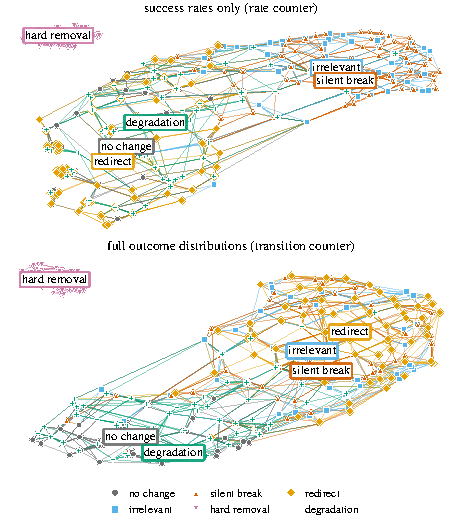
\includegraphics[width=\linewidth]{figures/fig_evidence_k10.pdf}
\caption{Evidence neighborhoods of all instances at $K = 10$.}
\label{fig:evidence}
\end{figure}

\Cref{fig:evidence} shows what each kind of evidence makes visible. Every point is one eight-node instance at $K = 10$, placed by the statistics a reference reads from the prompt and linked to its nearest neighbors. Position shows how similar the evidence is, and the axes have no units. Of a redirect instance's nearest neighbors, \redirNbNoChangeRate{} percent are no change instances and \redirNbBreakRate{} percent are silent breaks or irrelevant edits when only success rates are read. From full outcome distributions the redirect instances join the single-link breaks (\redirNbNoChangeTrans{} and \redirNbBreakTrans{} percent). Silent break and irrelevant overlap in both panels because they leave the same trace and differ only in relevance, and hard removal is read from the menus.

Intervals are 95 percent Wilson intervals over the \nSeedsEight{} seeds. \Cref{fig:evidenceK} repeats \cref{fig:evidence} at the other two budgets. In these embeddings only the neighbor links and the grouping are meaningful, not distances between groups.

\begin{figure}[!htb]
\centering
\begin{tikzpicture}
\begin{axis}[
    width=\linewidth, height=5.4cm,
    xmode=log, log basis x=2,
    xtick={5,10,20}, xticklabels={5,10,20},
    xmin=4.2, xmax=24, ymin=-0.04, ymax=1.06,
    ytick={0,0.25,0.5,0.75,1},
    yticklabel style={/pgf/number format/fixed, /pgf/number format/precision=2},
    xlabel={Attempts per pair in each period, $K$},
    ylabel={Localization accuracy},
    axis lines=left, tick style={draw=ecMuted}, axis line style={draw=ecMuted},
    label style={font=\small}, tick label style={font=\small},
    ymajorgrids, grid style={draw=ecLine!50, line width=0.3pt},
    legend columns=2, legend style={font=\scriptsize, draw=none, fill=none, at={(0.5,-0.32)}, anchor=north, cells={anchor=west}, column sep=4pt, row sep=-1pt},
    every axis plot/.append style={line width=1.0pt, mark size=2pt, error bars/y dir=both, error bars/y explicit, error bars/error bar style={line width=0.5pt}},
  ]
  \addplot[color=ecControl, dashed, mark=o, mark options={solid}] coordinates {\bcRateStoSilentbreakCI};
  \addlegendentry{silent break, rate}
  \addplot[color=ecControl, mark=*] coordinates {\bcGenStoSilentbreakCI};
  \addlegendentry{silent break, gen.}
  \addplot[color=ecControl!55, dashed, mark=triangle, mark options={solid}] coordinates {\bcRateStoDegradationCI};
  \addlegendentry{degradation, rate}
  \addplot[color=ecControl!55, mark=triangle*] coordinates {\bcGenStoDegradationCI};
  \addlegendentry{degradation, gen.}
  \addplot[color=ecTarget, dashed, mark=otimes, mark options={solid}] coordinates {\bcRateStoRedirectCI};
  \addlegendentry{redirect, rate}
  \addplot[color=ecTrans, mark=square*] coordinates {\bcGenStoRedirectCI};
  \addlegendentry{redirect, gen.}
\end{axis}
\end{tikzpicture}
\caption{Localization accuracy of two references.}
\label{fig:counters}
\end{figure}
\begin{figure*}[t]
\centering
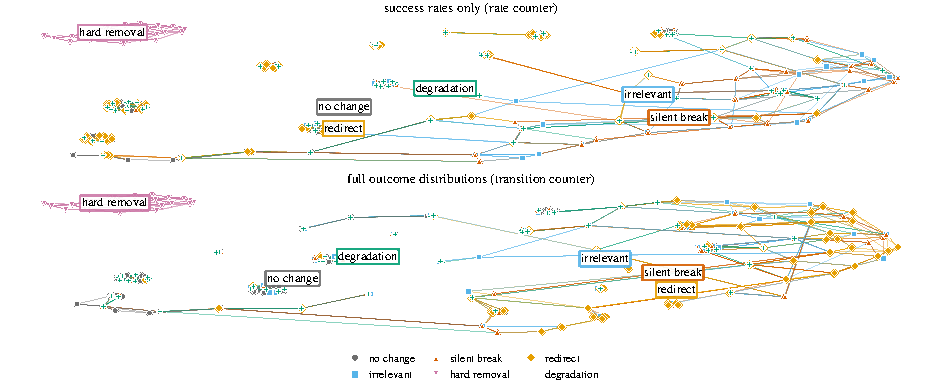
\includegraphics[width=0.49\textwidth]{figures/fig_evidence_k5.pdf}\hfill
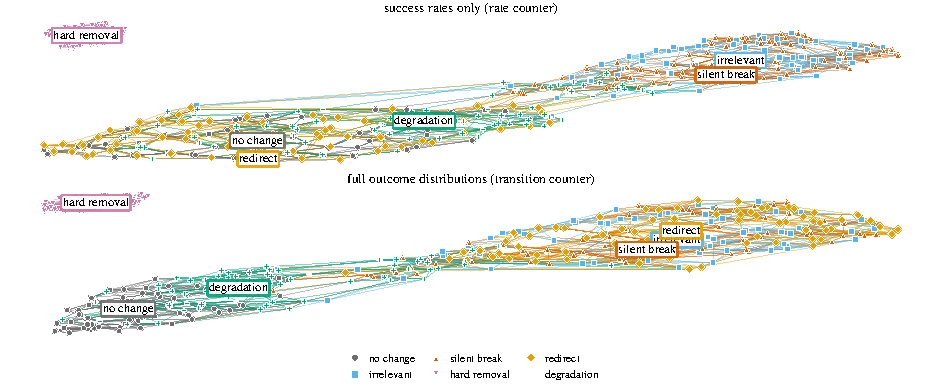
\includegraphics[width=0.49\textwidth]{figures/fig_evidence_k20.pdf}
\caption{Evidence neighborhoods at $K = 5$ (left) and $K = 20$ (right).}
\label{fig:evidenceK}
\end{figure*}

\paragraph{Evidence collection.}\label{app:evidence}
A fixed policy that does no reasoning collects the evidence separately in each world. Episodes start at random nodes, and at every node the policy attempts the least-tried listed action, breaking ties at random, until every listed pair has at least $K$ attempts. The data budget is thus set per node-action pair rather than per episode, and the per-pair counts are stored so the balance can be verified. A single function builds this prompt-safe view, and it never passes the per-pair counts, the worlds, the change record or the oracle into a prompt. The prompt then shows exactly $K$ events per pair, drawn uniformly from the collected events without regard to their outcome.

\paragraph{Runs.}\label{app:runs}
All confirmatory runs use seeds 31 to 130. On every model the eight-node family runs in the stochastic mode in the two-turn protocol, on all conditions at $K = 10$ and on silent break, degradation and no change at $K = 5$ and $K = 20$. Silent break and no change also run in the Single-turn setting, with the counts given, with minimal logs, and without the keep-destination rule. The sixteen-node family runs in the two-turn protocol at $K = 10$ on silent break and no change, and the deterministic mode on all conditions. The agentic arm runs on the first \nAgentic{} confirmatory seeds with stochastic silent break (\cref{sec:res-agentic}). Each instance is answered once, at temperature 0 where the provider allows it. GPT-5.6 Sol and Kimi K2.7 Code reason by default and run at their providers' settings (\cref{tab:models}). Answer variance and parse failures are treated in \cref{app:method}.

\paragraph{Models.}
\Cref{tab:models} lists the model settings. Providers can reuse a short model name for newer releases, so a short name does not identify one model over time. The DeepSeek row gives the case that affects this study.

\begin{table}[!htb]
\centering
\scriptsize
\caption{Model settings.}
\label{tab:models}
\begin{tabularx}{\linewidth}{@{}l >{\raggedright\arraybackslash}X@{}}
\toprule
Model & Settings \\
\midrule
Gemma 4 E4B & \texttt{google/gemma-4-E4B-it}, local, temperature 0. Quantization \mGemmaQuant{}, runtime \mGemmaRuntime{}, run \mAccessGemma{}. \\
GPT-4o & \texttt{gpt-4o}, temperature 0. Snapshot \mGPTfourSnapshot{}, accessed \mAccessGPTfour{}. \\
GPT-5.6 Sol & \texttt{gpt-5.6-sol}, reasoning effort medium (the API default), provider temperature, three answers per silent-break instance. Accessed \mAccessSol{}. \\
DeepSeek V4 Flash & checkpoint \texttt{DeepSeek-V4-Flash-0731}, requested explicitly because the API name \texttt{deepseek-v4-flash} now routes to V4.1 Flash. Thinking \mDeepSeekThinking{}, provider \mDeepSeekProvider{}, accessed \mAccessDeepSeek{}. \\
Kimi K2.7 Code & \texttt{kimi-k2.7-code}, thinking always on, provider temperature. Accessed \mAccessKimi{}. \\
\bottomrule
\end{tabularx}
\end{table}

\paragraph{Hypothesis conditions.}\label{app:hypconditions}
H1 compares a plan with the model's own statement. Since a silently broken link stays on the menu, its condition reduces to the stated probability. It is measured without the keep-destination rule, which could itself pull the link into the plan, and is tested for a model only with at least 10 qualifying instances. Its denominators are selected by the model's own beliefs, so it supports no comparison across models. H4 counts only choices after six consecutive failures, when a generator-aware observer puts more than 95 percent on the link being broken, so rational retries do not count. The threshold 0.10 is a smallest effect of interest, with 0.05 and 0.20 as a sensitivity check. A positive H2 shows that tabulation helps, not that failures are tallying failures, since the tabulated view also changes format and length. A null result licenses no conclusion.

H6 compares the model\_first and task\_only conditions of the agentic arm on the same seeds, using H4's measure. It predicts a direction only, so it has no threshold. The smallest difference it can detect is computed from the variance of the confirmatory runs and reported with the result.

\paragraph{Analysis rules.}
(1) Seeds 1 to 30 are excluded from every confirmatory analysis. (2) The seed is the unit of analysis, with one answer per instance. The stability check is reported separately. (3) Hypotheses are one-sided, and each forms its own family across the five models. Differences are paired over seeds with 95\% percentile bootstrap intervals (10{,}000 resamples) and one-sided bootstrap $p$-values with Holm correction, and rates get one-sided Wilson lower bounds~\cite{wilson1927} with Bonferroni correction. Descriptive contrasts are not corrected and support no claim. There is no equivalence reading. As a rough guide only, since the exploratory run used an earlier protocol, \nSeedsEight{} paired seeds with Holm correction across five models and that run's standard deviation of paired differences (0.48) detect a difference of about \mdePaired{} at 80\% power. For H4, \nAgentic{} runs give 80\% power to show a lower bound above 0.10 when the true rate is 0.25, after Bonferroni correction across five models. (4) H1 is tested for a model only with at least 10 qualifying instances. H4 is tested only with at least 10 runs that reach six consecutive failures, and H6 only with at least 10 such runs in both conditions. (4b) A parse failure gets one repair request with the same wording for every model. If it still fails, it counts as incorrect, and results excluding such instances are reported beside. (4c) GPT-5.6 Sol, which runs at provider temperature, answers all silent-break instances three times, and every other model answers 10 seeds three times, to measure answer variance. (4d) The threshold 0.10 in H1 and H4 is a smallest effect of interest. An agent acting on its own statement, or on six straight failures, should almost never choose that link. (5) Detection thresholds come from the held-out calibration above. (6) The primary routing measure is the optimal-route rate over all instances. Deterministic routing is descriptive. (7) In the primary analysis a parse failure counts as incorrect. Results excluding parse failures are secondary. (8) No model is said to fail where no reference succeeds, models are not ranked, and no cell appears in a summary sentence without its $n$. The full plan is part of the supplementary material.

\paragraph{Reproducibility.}
The environment, the generator, the parser and the probe scorers are frozen at a tagged version, and every artifact records the frozen commit, the commit that produced it and whether the two match. Each artifact keeps the prompt-safe payload, the raw model response, the parser and execution statuses, the route and regret outputs, the seeds and model settings, and the realized event and token counts. The seed list is generated from the eligibility criteria rather than written by hand, so the two cannot drift. All code and run artifacts are public~\cite{ecpm2026}.

\paragraph{Supplementary material.} An extended methodology (theoretical grounding, evidence formats and assistance levels, the exploratory protocols, all pilot runs, the seed audit over seeds 1 to 30 and the finetuning arm) is part of the supplementary material, with the analysis plan, the code and all run artifacts~\cite{ecpm2026}.
% ===== end sections/appendix_a_methodology.tex =====

% ===== begin sections/appendix_b_pilots.tex =====
\subsection{Notation}\label{app:notation}
\Cref{tab:notation} lists the symbols used in the paper.

\begin{table}[!htb]
\centering
\small
\begin{tabular}{@{}l>{\raggedright\arraybackslash}p{0.56\linewidth}@{}}
\toprule
Symbol & Meaning \\
\midrule
$M_0$, $M_1$ & pre-change and post-change world \\
$S$, $A_w(s)$ & nodes, actions available at $s$ in $M_w$ \\
$d_w(s,a)$, $p_w(s,a)$ & destination and success probability \\
$p_{uv}$ & $p_w(u,a)$ for the action with $d_w(u,a)=v$ \\
$s_{\mathrm{start}}$, $g$ & start node and goal \\
$C(r)$, $\mathrm{regret}(r)$ & expected cost and regret of route $r$ \\
$N_g$ & attempts until the goal is reached \\
$\Tstar$, $\Ustar$ & on-route target and off-route control \\
$\mathcal{D}$, $\mathcal{R}$ & separating pairs, pairs on one menu only \\
$K$ & minimum attempts per pair and period \\
$\tau$ & tolerance for a stated probability \\
$\hat{p}$ & a stated success probability \\
$E_0$, $E_1$, $H$ & episodes per phase, step budget \\
$T_{w,e}$, $s_{w,e,t}$ & episode duration, node after $t$ attempts \\
$o_{w,e,t}$, $h_{w,e,t}$ & observation, history up to it \\
$\pi_\theta$ & the model's action-selection policy \\
\bottomrule
\end{tabular}
\caption{Symbols used in the paper.}
\label{tab:notation}
\end{table}

\FloatBarrier
\section{Pilot study and protocol revisions}\label{app:pilots}\label{sec-pilots}

\noindent One exploratory run at scale preceded the main runs. It is reported here and used for no confirmatory claim. Smaller pilots on one to three seeds are in the supplementary material. The exploratory run used seeds 1 to 30, which are therefore excluded from every confirmatory analysis.

\subsection{Exploratory GPT-4o run}

The one exploratory run at scale used GPT-4o with an earlier protocol, in which the model reported beliefs about four queried pairs and answered the Period B probes as successive questions, on the 23 eligible seeds among seeds 1 to 30, stochastic mode, $K = 10$, with shuffled triples, temperature 0, belief re-elicitation and one sample per instance, on three conditions (69 instances). Every probe parsed. \Cref{tab-gpt4o} gives the results, with Wilson 95 percent intervals in brackets. Localization is not asked under no change.

\begin{table*}[t]
\centering
\small
\caption{Exploratory GPT-4o run.}
\label{tab-gpt4o}
\begin{tabular}{@{}llll@{}}
\toprule
Measure & No change & Irrelevant & Silent break \\
\midrule
Detection, correct & 18/23 & 10/23 & 11/23 \\
Localization & (not asked) & 9/23 [0.22, 0.59] & 6/23 [0.13, 0.46] \\
Preservation, mean & 0.924 & 0.772 & 0.696 \\
Preservation, all four correct & 20/23 & 9/23 & 6/23 \\
Self-consistency Preservation, mean & 0.902 & 0.870 & 0.848 \\
Route-taking (B), valid & 18/23 & 16/23 & 15/23 \\
Route-taking (B), optimal & 5/23 [0.10, 0.42] & 4/23 [0.07, 0.37] & 9/23 [0.22, 0.59] \\
Route-taking (B), mean regret & 1.248 & 0.787 & 0.505 \\
\bottomrule
\end{tabular}
\end{table*}

On silent break GPT-4o detected the change in \exSBDet{} of \exN{} instances and localized it in \exSBLoc, below the baseline's 0.96 at the same $K$, while false alarms on no change stayed at \exNCFalse{} of \exN. Crossing Localization with an optimal Period B route gives \exCellLocOpt, \exCellLocOnly, \exCellOptOnly{} and \exCellNeither{} instances (localized and optimal, localized only, optimal only, neither). The odds ratio is \exOR{} [\exORlo, \exORhi] with Fisher $p = \exFisherP$, and on no change only \exNCRouteOpt{} of \exN{} routes were optimal, so low route optimality alone fills the discordant cells.

% ---------------------------------------------------------------------------

\subsection{Design changes before the confirmatory runs}
The analysis plan was revised after the exploratory run, after internal review, and when the model-first conditions were added to the agentic arm, each time before any confirmatory data existed. \Cref{tab:changes} lists each change and its reason. The plan itself is in the supplementary material. A cost comparison, giving tokens, wall time, price and storage per instance for each model and CPU time for the references, is reported as exploratory and tests no hypothesis.

\begin{table*}[h]
\centering
\small
\caption{Design changes before the confirmatory runs.}
\label{tab:changes}
\begin{tabularx}{\textwidth}{@{}>{\raggedright\arraybackslash}p{0.36\textwidth} >{\raggedright\arraybackslash}X@{}}
\toprule
Change & Reason \\
\midrule
Five queried pairs, one Period B answer & Preservation shared a pair with Localization \\
Target queried on half of the seeds & always querying it narrowed the model's candidates, not the references' \\
Irrelevant control sets $\Ustar$ to $p = 0$ & a halved off-route link is not reliably localized at $K = 10$ \\
Thresholds calibrated on held-out seeds & first calibrated on the evaluated instances (0.50 at $K = 10$, with \pctOldFalseAlarm{} percent false alarms) \\
Transition counter, Bayesian and generator-aware observers & the rate counter cannot see redirect \\
Optimal-route rate over all instances. Parse failures incorrect & mean regret over valid routes favoured invalid routes \\
Noise band for stochastic Preservation & sampling noise exceeds $\tau$ on over a third of healthy pairs \\
Equivalence reading dropped & its margin had been widened from $\pm 0.20$ to $\pm 0.30$ after the exploratory run \\
H6 and the model\_first and graph\_given agentic conditions added & the model-first question was raised for the agentic arm. No confirmatory agentic data existed \\
Seeds 31 to 130, one answer each & seeds 1 to 30 were exploratory. Seeds, not samples, are the unit \\
H1 on the model's own belief, without the keep-destination rule & conditioning on correct Localization, and the rule, could each produce the effect \\
H4 counted after six consecutive failures & earlier counting penalized rational retries \\
H5 added. Deterministic mode descriptive & the gap question was untested. Ties on most deterministic seeds \\
\bottomrule
\end{tabularx}
\end{table*}
% ===== end sections/appendix_b_pilots.tex =====

% ===== begin sections/appendix_c_analysis_plan.tex =====
\section{Agentic exploration details}\label{sec-agentic}\label{app:agentic}

\paragraph{Interaction model.}\label{app:interaction}
Let $s_{w,e,t}$ denote the node occupied after $t$ attempts in episode $e$ of phase $w\in\{0,1\}$. An episode ends when the goal is reached or the budget is exhausted, so its duration is
\[
T_{w,e} = \min\left\{H,\, \inf\{t\geq 0:s_{w,e,t}=g\}\right\},
\]
with the inner infimum taken as $+\infty$ if the goal is never reached.

Before each action, the model receives its current node, the available action labels, the remaining step budget, and feedback about the preceding attempt.
For episode $e$ in phase $w$, we write this observation as
\[
o_{w,e,t}
=
\left(
s_{w,e,t},
A_w(s_{w,e,t}),
H-t,
f_{w,e,t}
\right),
\]
for $t=0,\ldots,T_{w,e}-1$, where $H$ is the episode's step budget and $f_{w,e,t}$ contains the preceding outcome feedback or an empty
value at the beginning of the episode. At the transition to $M_1$, an additional message tells the model that it has been placed back at the start. In the announced variant, the message adds that the link reliabilities may have changed. The main runs use the unannounced message. The interaction is maintained as a growing conversation so that each observation and the model's action response are appended. The outcome of the action chosen by the model is reported in the next observation, or in an additional message when the episode ends.
At each decision, the model receives the preceding conversation, including actions and outcomes from earlier episodes.

Let $h_{w,e,t}$ denote this conversation up to and including the current observation. The model induces a
history-dependent action-selection policy
\[
a_{w,e,t}
\sim
\pi_\theta(\,\cdot\mid h_{w,e,t}),
\]
where $\theta$ denotes the fixed model parameters.
For an available action, the next step is sampled
\[
s_{w,e,t+1}
\sim
P_w(\,\cdot\mid s_{w,e,t},a_{w,e,t}).
\]
An action outside the current menu consumes one step, leaves the packet at its current node and is answered with a message that the action is not available. Only a reply that cannot be read as an action is returned for correction, at most twice, after which the episode ends.

The model learns about the environment through the
interaction history. A failed available action consumes one
step and leaves the packet at its current node.
A successful action consumes one step and reveals its
destination through the next observed node.

\paragraph{Configuration.}
The main runs use the first \nAgentic{} confirmatory seeds, stochastic silent break, four $M_0$ and four $M_1$ episodes of at most 25 steps, with the unannounced transition message, for every model. Afterwards the model answers the probes on a copy of its own transcript. The interaction history is retained across episodes and phases. The oldest turns are trimmed only when the transcript exceeds an estimated 12{,}000 tokens, never below the six most recent turns. Every trim that removes an observation of the target is logged, and the share of runs affected is reported. At every step the model may reason briefly in prose, but it must end its reply with one JSON object naming a single action, and the last such object in the reply is taken. A readable choice of an action outside the menu is not a format error and costs one step (\cref{app:interaction}). Runs record this action protocol so that they are not pooled with runs made under the earlier rule, in which such a choice was returned for a free correction.

\paragraph{Behavioral metrics.}
Goal success rate is the share of episodes in a phase that reach the goal, counting step-limit cutoffs and parser aborts as failures. Steps to goal is the mean and median over goal-reaching episodes. Optimal action rate is the share of decisions that match an optimal action, averaged per episode, so each episode weighs equally. Parse failures are instead pooled over every step, so long episodes weigh more in that rate. An unavailable action counts as a non-optimal decision and consumes a step. Route regret is the regret of the realized route by \cref{eq:regret}, unrounded and averaged over goal-reaching episodes.

Changed-action usage is the share of decisions at the source node of the changed pair that choose the changed action, reported for $M_0$, for $M_1$, and after the first feedback that reveals the change. That feedback is the first failed $M_1$ attempt of the changed action under silent break, degradation and the irrelevant control. The first successful move to a destination other than the one observed in $M_0$ under redirect, and the first $M_1$ visit to the source node after an $M_0$ visit under hard removal. It marks evidence available to the model, not recognition, and in the stochastic mode a single failure does not prove a change. Changed-action switch is the number of decisions at the source node after that feedback, up to and including the first choice of a legal alternative, so a switch at the first opportunity has lag one. A first switch does not establish sustained adaptation.

The $M_0$ observation reference is built only from the transitions the model itself observed in $M_0$, with observed destinations and Laplace-smoothed success probabilities, so no hidden topology enters it, and it is distinct from the evaluator's full simulator. $M_1$ choices are scored against its best known routes. Decisions it cannot score are skipped and counted by reason, and agreement is averaged over the evaluable decisions of each episode.

\paragraph{Hypothesis H4 and reference agent.}
H4 counts the choices of the broken link made after six consecutive observed failures of it, over all runs and, secondarily, over runs that localize the break. An evidence-only reference agent runs in the same arm. It routes by Dijkstra's algorithm on the posterior mean success probabilities under the generator's prior, avoids a link once its posterior of being broken exceeds 0.95, and gives the reference adaptation lag, the number of steps from the first observed failure of the broken link to the last attempt at it.

\paragraph{Pilot.}
In a pilot run on seed 7 with a silent break, under the earlier action protocol, GPT-5.6 Sol answered all four probes correctly, yet after the broken link first failed it kept choosing it on later visits to that node. It reported the change correctly without acting on it. This is one pilot instance and motivates the arm. \Cref{tab:verdicts-full} gives the confirmatory H4 and H6 results for each model. Over all confirmatory runs the adaptation lag is \RES{} steps, against a median of \lagRefAgent{} for the reference agent.
% ===== end sections/appendix_c_analysis_plan.tex =====

% ===== begin sections/appendix_d_prompts.tex =====
\section{Prompt templates}\label{app:prompts}

The text sent to the model in the two-turn protocol, for stochastic silent break at $K = 10$ on the first confirmatory seed (seed 33), is reproduced below with the evidence records shortened. Every other part is verbatim. The full prompts of every run are stored with its artifact~\cite{ecpm2026}. Turn 2 shows the confirmatory Period B schema, which asks for a belief about every listed pair.

\paragraph{Turn 1 (Period A).}
% prompt-source: turn_A
{\scriptsize
\begin{verbatim}
Period A.
Each action has one destination. A successful
attempt moves to that destination. A failed
attempt leaves the system at the current node,
and the action can be retried. Each attempt
costs 1.
destination is the non-current node reached on a
successful attempt. A destination is always
different from the current node. Count an
observation as a success exactly when its next
node differs from its current node. p_success is
the fraction of visible observations counted as
successes. If an available action has no
successful observations in the current period,
keep its most recent earlier destination
estimate if one exists; otherwise use null.

Nodes: A, B, C, D, E, F, G, H
Start: E   Goal: C
Action menu, Period A: A: a1, a2; B: a1, a2; D:
a1, a2, a3; E: a1, a2; F: a1, a2; G: a1, a2; H:
a1, a2

Raw shuffled observations, Period A:
[D, a3, D]
[B, a2, E]
[B, a1, F]
[A, a2, F]
[F, a2, F]
[B, a1, F]
[... 144 further records ...]

Pairs to report in this order:
- B a1
- B a2
- D a3
- F a1
- G a2

Return exactly one JSON object with exactly five
pairs:
{
  "pairs": [
    {"node": "<node>", "action": "<action>",
"available": <boolean>,
     "destination": "<node or null>",
"p_success": <number or null>}
  ],
  "route": [{"node": "<node>", "action":
"<action>"}]
}
For each listed pair, available means that the
action appears in the current
menu; it does not mean the action works. A route
lists actions only. Its first item must be at
Start. The successful destination of its final
action must be Goal. Do not add a route item for
Goal after arrival. Do not include other text.
\end{verbatim}}

\paragraph{Turn 2 (Period B added).}
% prompt-source: turn_B
{\scriptsize
\begin{verbatim}
Period B may or may not differ from Period A.
Each action has one destination. A successful
attempt moves to that destination. A failed
attempt leaves the system at the current node,
and the action can be retried. Each attempt
costs 1.
destination is the non-current node reached on a
successful attempt. A destination is always
different from the current node. Count an
observation as a success exactly when its next
node differs from its current node. p_success is
the fraction of visible observations counted as
successes. If an available action has no
successful observations in the current period,
keep its most recent earlier destination
estimate if one exists; otherwise use null.

Nodes: A, B, C, D, E, F, G, H
Start: E   Goal: C
Action menu, Period B: A: a1, a2; B: a1, a2; D:
a1, a2, a3; E: a1, a2; F: a1, a2; G: a1, a2; H:
a1, a2

Raw shuffled observations, Period B:
[F, a1, E]
[H, a1, B]
[B, a1, B]
[G, a1, E]
[A, a2, F]
[E, a2, D]
[... 144 further records ...]

Pairs to report in this order:
- B a1
- B a2
- D a3
- F a1
- G a2
- A a1
- A a2
- D a1
- D a2
- E a1
- E a2
- F a2
- G a1
- H a1
- H a2

Return exactly one JSON object with every listed
pair:
{
  "changed": <boolean>,
  "changed_pair": <null or {"node": "<node>",
"action": "<action>"}>,
  "pairs": [
    {"node": "<node>", "action": "<action>",
"available": <boolean>,
     "changed": <boolean>,
     "destination": "<node or null>",
"p_success": <number or null>}
  ],
  "route": [{"node": "<node>", "action":
"<action>"}]
}
If changed is false, changed_pair must be null.
If changed is true,
changed_pair must name the one pair judged to
have changed. For each listed
pair, available means that the action appears in
the Period B menu; it does
not mean the action works. If an action is
unavailable, use available=false,
destination=null, and p_success=null. A route
lists actions only. Its first item must be at
Start. The successful destination of its final
action must be Goal. Do not add a route item for
Goal after arrival. Do not include other text.
\end{verbatim}}

\paragraph{Agentic arm.}
The system prompt, an example step observation and the transition message to $M_1$, as sent by the harness. \texttt{<goal>}, the node, the menu and the step count are filled in per step.
% prompt-source: agent_system
{\scriptsize
\begin{verbatim}
You are exploring an unfamiliar courier network
of locations connected by one-way links. At each
location you may attempt one of the listed
actions (aK). An attempt either delivers you to
that action's destination, or fails and you stay
where you are -- either way it costs one step.
You do not know the network's structure or
reliabilities in advance: you must learn them by
trying actions and observing what happens. Your
goal is to reach <goal> in as few steps as
possible, across several episodes. The network's
reliabilities may or may not change between
episodes; nothing will tell you this directly --
watch your own outcomes. For every step: you may
reason briefly first, but end your reply with
exactly one JSON object of the form {"action":
"aK"} naming the single action you choose.
Output no other JSON object in your reply.
\end{verbatim}}

\noindent Step observation:
% prompt-source: agent_step
{\scriptsize
\begin{verbatim}
Your last action a1 failed (you stayed).
You are at B. Steps remaining this episode: 22.
Legal actions here: a1, a2.
Choose one. End your reply with exactly one JSON
object: {"action": "aK"}.
\end{verbatim}}

\noindent Transition to $M_1$, main runs, and announced variant:
% prompt-source: agent_transition
{\scriptsize
\begin{verbatim}
You are placed back at the start. Continue.

You are placed back at the start. The network's
link reliabilities may have changed since your
last episode.
\end{verbatim}}

\noindent In the model\_first condition the system prompt ends with the sentence below, and before every episode after the first the model receives the first request below (later episodes: the second).
% prompt-source: agent_system_model_first_suffix
{\scriptsize
\begin{verbatim}
Between episodes you will also be asked to
describe your current model of the network; that
reply needs no JSON object.
\end{verbatim}}

% prompt-source: agent_model_first_requests
{\scriptsize
\begin{verbatim}
Before the next episode, construct a model of
how this network behaves from what you have
observed so far. Use whatever representation you
find useful. Describe the current network so
that your model can be used to choose actions
later. Reply in free text; do not include a JSON
object.

Before the next episode, update your model of
how this network behaves using everything you
have observed so far. Use whatever
representation you find useful. Describe the
current network so that your model can be used
to choose actions later. Reply in free text; do
not include a JSON object.
\end{verbatim}}
% ===== end sections/appendix_d_prompts.tex =====

% ===== begin sections/appendix_e_full_results.tex =====
\section{Future work}\label{app:future}
A finetuning arm, in which the same observation log is written into the weights rather than the prompt, would ask whether evidence absorbed by training is usable at all. For simulating online communities, fine-tuning on their own text has given more faithful models than in-context examples~\cite{chu2025}. Its harness exists but is not evaluated here. Other directions include coherence metrics in the style of \citet{vafa2024}, an environment described in natural language, and the questions of plasticity, catastrophic forgetting and curriculum order that arise when the periods are shown together or one after the other.
% (Future work above comes from sections/07_discussion.tex.)

\section{Additional results}\label{app:full}

The target is among the queried pairs on \nQueriedTarget{} of the \nQueriedSeeds{} seeds. On those seeds, restricted to the queried pairs, the references localize between \qrRate{} (rate counter) and \qrGen{} (generator-aware observer) of silent breaks at $K = 10$.

\Cref{tab:n16} gives the core results for the sixteen-node family, which was run on silent break and no change, and \cref{tab:det} for the deterministic mode of the eight-node family, in the layout of \cref{tab:main}.
\Cref{tab:gap} gives the gap to the generator-aware observer at each $K$ (\cref{sec:res-evidence}), and \cref{tab:belief} crosses each model's stated belief about the broken link with its route use (\cref{sec:res-belief}).

\begin{table}[!htb]
\centering
\scriptsize
\caption{Gap to the generator-aware observer.}
\label{tab:gap}
\adjustbox{max width=\linewidth}{% ===== begin tables/h1_gap.tex =====
% Generated by scripts/make_tables.py. Do not edit by hand.
\begin{tabular}{@{}l ccc@{}}
\toprule
Model & $K{=}5$ & $K{=}10$ & $K{=}20$ \\
\midrule
Gemma 4 E4B & \RES & \RES & \RES \\
GPT-4o & \RES & \RES & \RES \\
GPT-5.6 Sol & \RES & \RES & \RES \\
DeepSeek V4 Flash & \RES & \RES & \RES \\
Kimi K2.7 Code & \RES & \RES & \RES \\
\bottomrule
\end{tabular}
% ===== end tables/h1_gap.tex =====
}
\end{table}

\begin{table}[!htb]
\centering
\scriptsize
\caption{Own belief and route use.}
\label{tab:belief}
\adjustbox{max width=\linewidth}{% ===== begin tables/belief_use.tex =====
% Generated by scripts/make_tables.py. Do not edit by hand.
\begin{tabular}{@{}ll cc cc@{}}
\toprule
& & \multicolumn{2}{c}{States broken} & \multicolumn{2}{c}{States usable} \\
\cmidrule(lr){3-4} \cmidrule(lr){5-6}
Model & Prompt & uses & avoids & uses & avoids \\
\midrule
Gemma 4 E4B & no rule & \RES & \RES & \RES & \RES \\
 & rule & \RES & \RES & \RES & \RES \\
GPT-4o & no rule & \RES & \RES & \RES & \RES \\
 & rule & \RES & \RES & \RES & \RES \\
GPT-5.6 Sol & no rule & \RES & \RES & \RES & \RES \\
 & rule & \RES & \RES & \RES & \RES \\
DeepSeek V4 Flash & no rule & \RES & \RES & \RES & \RES \\
 & rule & \RES & \RES & \RES & \RES \\
Kimi K2.7 Code & no rule & \RES & \RES & \RES & \RES \\
 & rule & \RES & \RES & \RES & \RES \\
\bottomrule
\end{tabular}
% ===== end tables/belief_use.tex =====
}
\end{table}


\begin{table*}[h]
\centering
\small
\setlength{\tabcolsep}{3pt}
\caption{Sixteen-node family, stochastic mode, $K = 10$.}
\label{tab:n16}
\adjustbox{max width=\linewidth}{% ===== begin tables/main_results_n16.tex =====
% Generated by scripts/make_tables.py. Do not edit by hand.
\begin{tabular}{@{}ll cccc ccc ccc ccc ccc ccc@{}}
\toprule
& & \multicolumn{4}{c}{References} & \multicolumn{3}{c}{Gemma 4 E4B} & \multicolumn{3}{c}{GPT-4o} & \multicolumn{3}{c}{GPT-5.6 Sol} & \multicolumn{3}{c}{DeepSeek V4 Flash} & \multicolumn{3}{c}{Kimi K2.7 Code} \\
\cmidrule(lr){3-6} \cmidrule(lr){7-9} \cmidrule(lr){10-12} \cmidrule(lr){13-15} \cmidrule(lr){16-18} \cmidrule(lr){19-21}
Mode & Condition & Rate & Bayes & Gen. & Route & Loc & Pres & Route & Loc & Pres & Route & Loc & Pres & Route & Loc & Pres & Route & Loc & Pres & Route \\
\midrule
Stoch. & No change & -- & -- & -- & 0.70 & -- & \RES & \RES & -- & \RES & \RES & -- & \RES & \RES & -- & \RES & \RES & -- & \RES & \RES \\
Stoch. & Silent break & 0.95 & 0.96 & 1.00 & 0.79 & \RES & \RES & \RES & \RES & \RES & \RES & \RES & \RES & \RES & \RES & \RES & \RES & \RES & \RES & \RES \\
\midrule
Parse failures &  &  &  &  &  &  & \RES &  &  & \RES &  &  & \RES &  &  & \RES &  &  & \RES &  \\
\bottomrule
\end{tabular}
% ===== end tables/main_results_n16.tex =====
}
\end{table*}

\begin{table*}[h]
\centering
\small
\setlength{\tabcolsep}{3pt}
\caption{Deterministic mode, $K = 10$.}
\label{tab:det}
\adjustbox{max width=\linewidth}{% ===== begin tables/det_results.tex =====
% Generated by scripts/make_tables.py. Do not edit by hand.
\begin{tabular}{@{}ll cccc ccc ccc ccc ccc ccc@{}}
\toprule
& & \multicolumn{4}{c}{References} & \multicolumn{3}{c}{Gemma 4 E4B} & \multicolumn{3}{c}{GPT-4o} & \multicolumn{3}{c}{GPT-5.6 Sol} & \multicolumn{3}{c}{DeepSeek V4 Flash} & \multicolumn{3}{c}{Kimi K2.7 Code} \\
\cmidrule(lr){3-6} \cmidrule(lr){7-9} \cmidrule(lr){10-12} \cmidrule(lr){13-15} \cmidrule(lr){16-18} \cmidrule(lr){19-21}
Mode & Condition & Rate & Bayes & Gen. & Route & Loc & Pres & Route & Loc & Pres & Route & Loc & Pres & Route & Loc & Pres & Route & Loc & Pres & Route \\
\midrule
Det. & No change & -- & -- & -- & 1.00 & -- & \RES & \RES & -- & \RES & \RES & -- & \RES & \RES & -- & \RES & \RES & -- & \RES & \RES \\
Det. & Irrelevant & 1.00 & 1.00 & 1.00 & 1.00 & \RES & \RES & \RES & \RES & \RES & \RES & \RES & \RES & \RES & \RES & \RES & \RES & \RES & \RES & \RES \\
Det. & Silent break & 1.00 & 1.00 & 1.00 & 1.00 & \RES & \RES & \RES & \RES & \RES & \RES & \RES & \RES & \RES & \RES & \RES & \RES & \RES & \RES & \RES \\
Det. & Hard removal & 1.00 & 1.00 & 1.00 & 1.00 & \RES & \RES & \RES & \RES & \RES & \RES & \RES & \RES & \RES & \RES & \RES & \RES & \RES & \RES & \RES \\
Det. & Redirect & 0.10 & 1.00 & 1.00 & 1.00 & \RES & \RES & \RES & \RES & \RES & \RES & \RES & \RES & \RES & \RES & \RES & \RES & \RES & \RES & \RES \\
\midrule
Parse failures &  &  &  &  &  &  & \RES &  &  & \RES &  &  & \RES &  &  & \RES &  &  & \RES &  \\
\bottomrule
\end{tabular}
% ===== end tables/det_results.tex =====
}
\end{table*}


\Cref{tab:verdicts-full} gives every contrast of \cref{tab:hyp} per model and mode: the paired difference over seeds, its 95\% bootstrap interval, the Holm-adjusted $p$, the number of seeds, and the verdict. For H1 the estimate is a count with a Wilson interval, and the reference row gives the same share among instances where the model states that the link is usable.

\begin{table*}[h]
\centering
\small
\caption{All contrasts.}
\label{tab:verdicts-full}
% ===== begin tables/verdicts.tex =====
% Generated by scripts/make_tables.py. Do not edit by hand.
\begin{tabular}{@{}llrcrrl@{}}
\toprule
Hyp. & Model & Est. & Interval & $p_{\text{Holm}}$ & $n$ & Reading \\
\midrule
H1 & Gemma 4 E4B & 0/\RES & -- & -- & \RES & \RES \\
H1 & GPT-4o & 0/\RES & -- & -- & \RES & \RES \\
H1 & GPT-5.6 Sol & 0/\RES & -- & -- & \RES & \RES \\
H1 & DeepSeek V4 Flash & 0/\RES & -- & -- & \RES & \RES \\
H1 & Kimi K2.7 Code & 0/\RES & -- & -- & \RES & \RES \\
H1 (rule) & Gemma 4 E4B & 0/\RES & -- & -- & \RES & \RES \\
H1 (rule) & GPT-4o & 0/\RES & -- & -- & \RES & \RES \\
H1 (rule) & GPT-5.6 Sol & 0/\RES & -- & -- & \RES & \RES \\
H1 (rule) & DeepSeek V4 Flash & 0/\RES & -- & -- & \RES & \RES \\
H1 (rule) & Kimi K2.7 Code & 0/\RES & -- & -- & \RES & \RES \\
H1 (rule) ref. & Gemma 4 E4B & 0/\RES & -- & -- & \RES & states usable \\
H1 (rule) ref. & GPT-4o & 0/\RES & -- & -- & \RES & states usable \\
H1 (rule) ref. & GPT-5.6 Sol & 0/\RES & -- & -- & \RES & states usable \\
H1 (rule) ref. & DeepSeek V4 Flash & 0/\RES & -- & -- & \RES & states usable \\
H1 (rule) ref. & Kimi K2.7 Code & 0/\RES & -- & -- & \RES & states usable \\
H1 ref. & Gemma 4 E4B & 0/\RES & -- & -- & \RES & states usable \\
H1 ref. & GPT-4o & 0/\RES & -- & -- & \RES & states usable \\
H1 ref. & GPT-5.6 Sol & 0/\RES & -- & -- & \RES & states usable \\
H1 ref. & DeepSeek V4 Flash & 0/\RES & -- & -- & \RES & states usable \\
H1 ref. & Kimi K2.7 Code & 0/\RES & -- & -- & \RES & states usable \\
H2 & Gemma 4 E4B & \RES & \RES & \RES & \RES & \RES \\
H2 & GPT-4o & \RES & \RES & \RES & \RES & \RES \\
H2 & GPT-5.6 Sol & \RES & \RES & \RES & \RES & \RES \\
H2 & DeepSeek V4 Flash & \RES & \RES & \RES & \RES & \RES \\
H2 & Kimi K2.7 Code & \RES & \RES & \RES & \RES & \RES \\
H3 & Gemma 4 E4B & \RES & \RES & \RES & \RES & \RES \\
H3 & GPT-4o & \RES & \RES & \RES & \RES & \RES \\
H3 & GPT-5.6 Sol & \RES & \RES & \RES & \RES & \RES \\
H3 & DeepSeek V4 Flash & \RES & \RES & \RES & \RES & \RES \\
H3 & Kimi K2.7 Code & \RES & \RES & \RES & \RES & \RES \\
H4 & Gemma 4 E4B & \RES & \RES & -- & \RES & \RES \\
H4 & GPT-4o & \RES & \RES & -- & \RES & \RES \\
H4 & GPT-5.6 Sol & \RES & \RES & -- & \RES & \RES \\
H4 & DeepSeek V4 Flash & \RES & \RES & -- & \RES & \RES \\
H4 & Kimi K2.7 Code & \RES & \RES & -- & \RES & \RES \\
H5 & Gemma 4 E4B & \RES & \RES & \RES & \RES & \RES \\
H5 & GPT-4o & \RES & \RES & \RES & \RES & \RES \\
H5 & GPT-5.6 Sol & \RES & \RES & \RES & \RES & \RES \\
H5 & DeepSeek V4 Flash & \RES & \RES & \RES & \RES & \RES \\
H5 & Kimi K2.7 Code & \RES & \RES & \RES & \RES & \RES \\
H6 & Gemma 4 E4B & \RES & \RES & \RES & \RES & \RES \\
H6 & GPT-4o & \RES & \RES & \RES & \RES & \RES \\
H6 & GPT-5.6 Sol & \RES & \RES & \RES & \RES & \RES \\
H6 & DeepSeek V4 Flash & \RES & \RES & \RES & \RES & \RES \\
H6 & Kimi K2.7 Code & \RES & \RES & \RES & \RES & \RES \\
\bottomrule
\end{tabular}
% ===== end tables/verdicts.tex =====

\end{table*}

\Cref{tab:detection} reports sensitivity, the share of changed instances reported as changed, specificity, the share of no change instances reported as unchanged, and the discriminability $d'$ (log-linear corrected) for the three references and every model. 

\begin{table*}[h]
\centering
\scriptsize
\setlength{\tabcolsep}{2.5pt}
\caption{Detection at $K = 10$.}
\label{tab:detection}
\adjustbox{max width=\linewidth}{% ===== begin tables/detection.tex =====
% Generated by scripts/make_tables.py. Do not edit by hand.
\begin{tabular}{@{}l ccc ccc ccc ccc ccc ccc ccc ccc@{}}
\toprule
& \multicolumn{3}{c}{Rate} & \multicolumn{3}{c}{Trans.} & \multicolumn{3}{c}{Bayes} & \multicolumn{3}{c}{Gemma 4 E4B} & \multicolumn{3}{c}{GPT-4o} & \multicolumn{3}{c}{GPT-5.6 Sol} & \multicolumn{3}{c}{DeepSeek V4 Flash} & \multicolumn{3}{c}{Kimi K2.7 Code} \\
Mode & Sens & Spec & $d'$ & Sens & Spec & $d'$ & Sens & Spec & $d'$ & Sens & Spec & $d'$ & Sens & Spec & $d'$ & Sens & Spec & $d'$ & Sens & Spec & $d'$ & Sens & Spec & $d'$ \\
\midrule
Stoch. & 0.61 & 0.95 & 1.90 & 0.80 & 0.95 & 2.45 & 0.80 & 0.95 & 2.45 & \RES & \RES & \RES & \RES & \RES & \RES & \RES & \RES & \RES & \RES & \RES & \RES & \RES & \RES & \RES \\
Det. & 0.75 & 1.00 & 3.19 & 1.00 & 1.00 & 5.49 & 1.00 & 1.00 & 5.49 & \RES & \RES & \RES & \RES & \RES & \RES & \RES & \RES & \RES & \RES & \RES & \RES & \RES & \RES & \RES \\
\bottomrule
\end{tabular}
% ===== end tables/detection.tex =====
}
\end{table*}

\Cref{tab:ablations} gives, for each model on stochastic silent break, the share of seeds localized (Loc) and of optimal Period B routes (Route) in the core setting, at $K = 5$ and $K = 20$, with the counts given, with minimal logs, without the keep-destination rule, and in the Single-turn setting. Averaged over models, Localization changes by \RES{} from $K = 5$ to $K = 20$ and by \RES{} with the counts given. Removing the keep-destination rule changes the optimal-route rate by \RES, and the Single-turn setting changes it by \RES.

\begin{table*}[h]
\centering
\scriptsize
\setlength{\tabcolsep}{3pt}
\caption{Ablations.}
\label{tab:ablations}
\adjustbox{max width=\linewidth}{% ===== begin tables/ablations.tex =====
% Generated by scripts/make_tables.py. Do not edit by hand.
\begin{tabular}{@{}ll cc@{}}
\toprule
Model & Variant & Loc & Route \\
\midrule
Gemma 4 E4B & Core ($K{=}10$) & \RES & \RES \\
 & $K{=}5$ & \RES & \RES \\
 & $K{=}20$ & \RES & \RES \\
 & Counts given & \RES & \RES \\
 & Minimal logs & \RES & \RES \\
 & No keep-destination rule & \RES & \RES \\
 & Single-turn & \RES & \RES \\
\midrule
GPT-4o & Core ($K{=}10$) & \RES & \RES \\
 & $K{=}5$ & \RES & \RES \\
 & $K{=}20$ & \RES & \RES \\
 & Counts given & \RES & \RES \\
 & Minimal logs & \RES & \RES \\
 & No keep-destination rule & \RES & \RES \\
 & Single-turn & \RES & \RES \\
\midrule
GPT-5.6 Sol & Core ($K{=}10$) & \RES & \RES \\
 & $K{=}5$ & \RES & \RES \\
 & $K{=}20$ & \RES & \RES \\
 & Counts given & \RES & \RES \\
 & Minimal logs & \RES & \RES \\
 & No keep-destination rule & \RES & \RES \\
 & Single-turn & \RES & \RES \\
\midrule
DeepSeek V4 Flash & Core ($K{=}10$) & \RES & \RES \\
 & $K{=}5$ & \RES & \RES \\
 & $K{=}20$ & \RES & \RES \\
 & Counts given & \RES & \RES \\
 & Minimal logs & \RES & \RES \\
 & No keep-destination rule & \RES & \RES \\
 & Single-turn & \RES & \RES \\
\midrule
Kimi K2.7 Code & Core ($K{=}10$) & \RES & \RES \\
 & $K{=}5$ & \RES & \RES \\
 & $K{=}20$ & \RES & \RES \\
 & Counts given & \RES & \RES \\
 & Minimal logs & \RES & \RES \\
 & No keep-destination rule & \RES & \RES \\
 & Single-turn & \RES & \RES \\
\bottomrule
\end{tabular}
% ===== end tables/ablations.tex =====
}
\end{table*}

\Cref{tab:beliefacc} gives Period A belief accuracy for the five queried pairs: the share of beliefs correct on availability, destination and probability within $\tau$, destination accuracy alone, and the mean absolute error of the stated probability against the rate visible in the prompt.

\begin{table}[!htb]
\centering
\scriptsize
\caption{Period A belief accuracy.}
\label{tab:beliefacc}
\adjustbox{max width=\linewidth}{% ===== begin tables/belief_accuracy.tex =====
% Generated by scripts/make_tables.py. Do not edit by hand.
\begin{tabular}{@{}l ccc@{}}
\toprule
Model & Accuracy & Destination & Prob.\ MAE \\
\midrule
Gemma 4 E4B & \RES & \RES & \RES \\
GPT-4o & \RES & \RES & \RES \\
GPT-5.6 Sol & \RES & \RES & \RES \\
DeepSeek V4 Flash & \RES & \RES & \RES \\
Kimi K2.7 Code & \RES & \RES & \RES \\
\bottomrule
\end{tabular}
% ===== end tables/belief_accuracy.tex =====
}
\end{table}
% ===== end sections/appendix_e_full_results.tex =====


\end{document}